%!TEX root = ../report.tex

\chapter{Dataset creation}

\section{Overview of the dataset}
Since semantic segmentation using deep learning is framed as a pixelwise classification task, an image of dimensions H$\times$W$\times$C requires a ground truth of dimensions H$\times$W, where H and W are the height and width of the image in the dataset having C number of channels. 

The scope of the dataset is to include objects associated to RoboCup @Work. The selected 18 objects are shown in Figure \ref{Fig:objects}.

	\begin{figure}
		\centering
		\begin{subfigure}{.3\textwidth}
  			\centering
  			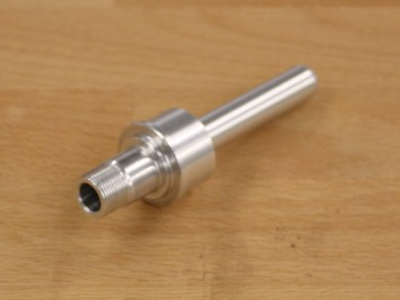
\includegraphics[width=.5\linewidth]{images/axis}
  			\caption{axis \cite{github_robocup@work}}
  			\label{fig:axis}
			\end{subfigure}%
		\begin{subfigure}{.3\textwidth}
  			\centering
  			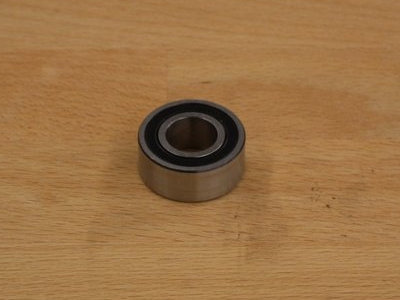
\includegraphics[width=.5\linewidth]{images/bearing}
  			\caption{bearing \cite{github_robocup@work}}
  			\label{fig:bearing}
		\end{subfigure}
		\begin{subfigure}{.3\textwidth}
  			\centering
  			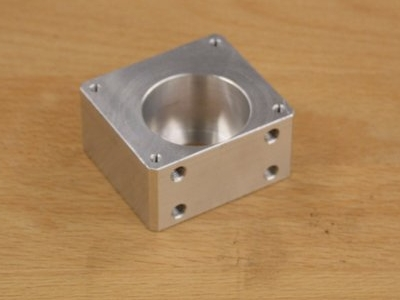
\includegraphics[width=.5\linewidth]{images/bearingBoxAX01}
  			\caption{bearing box AX01 \cite{github_robocup@work}}
  			\label{fig:bearingBoxAX01}
		\end{subfigure}\\
		\vspace{3mm}
		\begin{subfigure}{.3\textwidth}
  			\centering
  			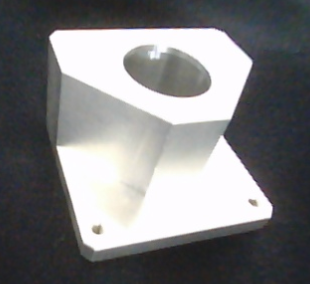
\includegraphics[width=.5\linewidth]{images/bearingBoxAX16}
  			\caption{bearing box AX16}
  			\label{fig:bearingBoxAX16}
		\end{subfigure}
		\begin{subfigure}{.3\textwidth}
  			\centering
  			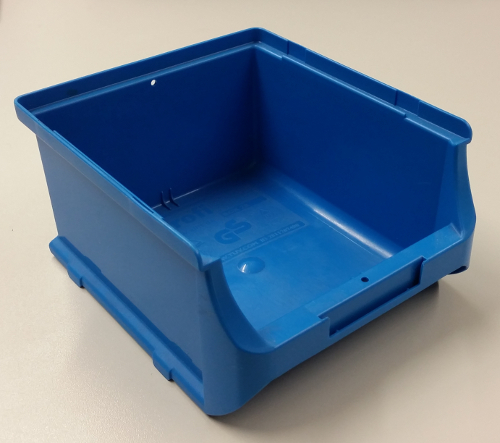
\includegraphics[width=.5\linewidth]{images/container_blue}
  			\caption{container blue \cite{github_robocup@work}}
  			\label{fig:container_blue}
		\end{subfigure}
		\begin{subfigure}{.3\textwidth}
  			\centering
  			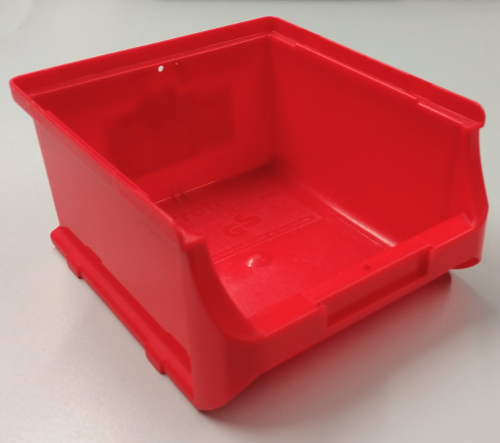
\includegraphics[width=.5\linewidth]{images/container_red}
  			\caption{container red \cite{github_robocup@work}}
  			\label{fig:container_red}
		\end{subfigure}\\
		\vspace{3mm}
		\begin{subfigure}{.3\textwidth}
  			\centering
  			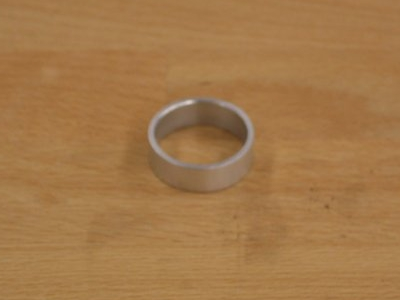
\includegraphics[width=.5\linewidth]{images/distanceTube}
  			\caption{distance tube \cite{github_robocup@work}}
  			\label{fig:distanceTube}
		\end{subfigure}
		\begin{subfigure}{.3\textwidth}
  			\centering
  			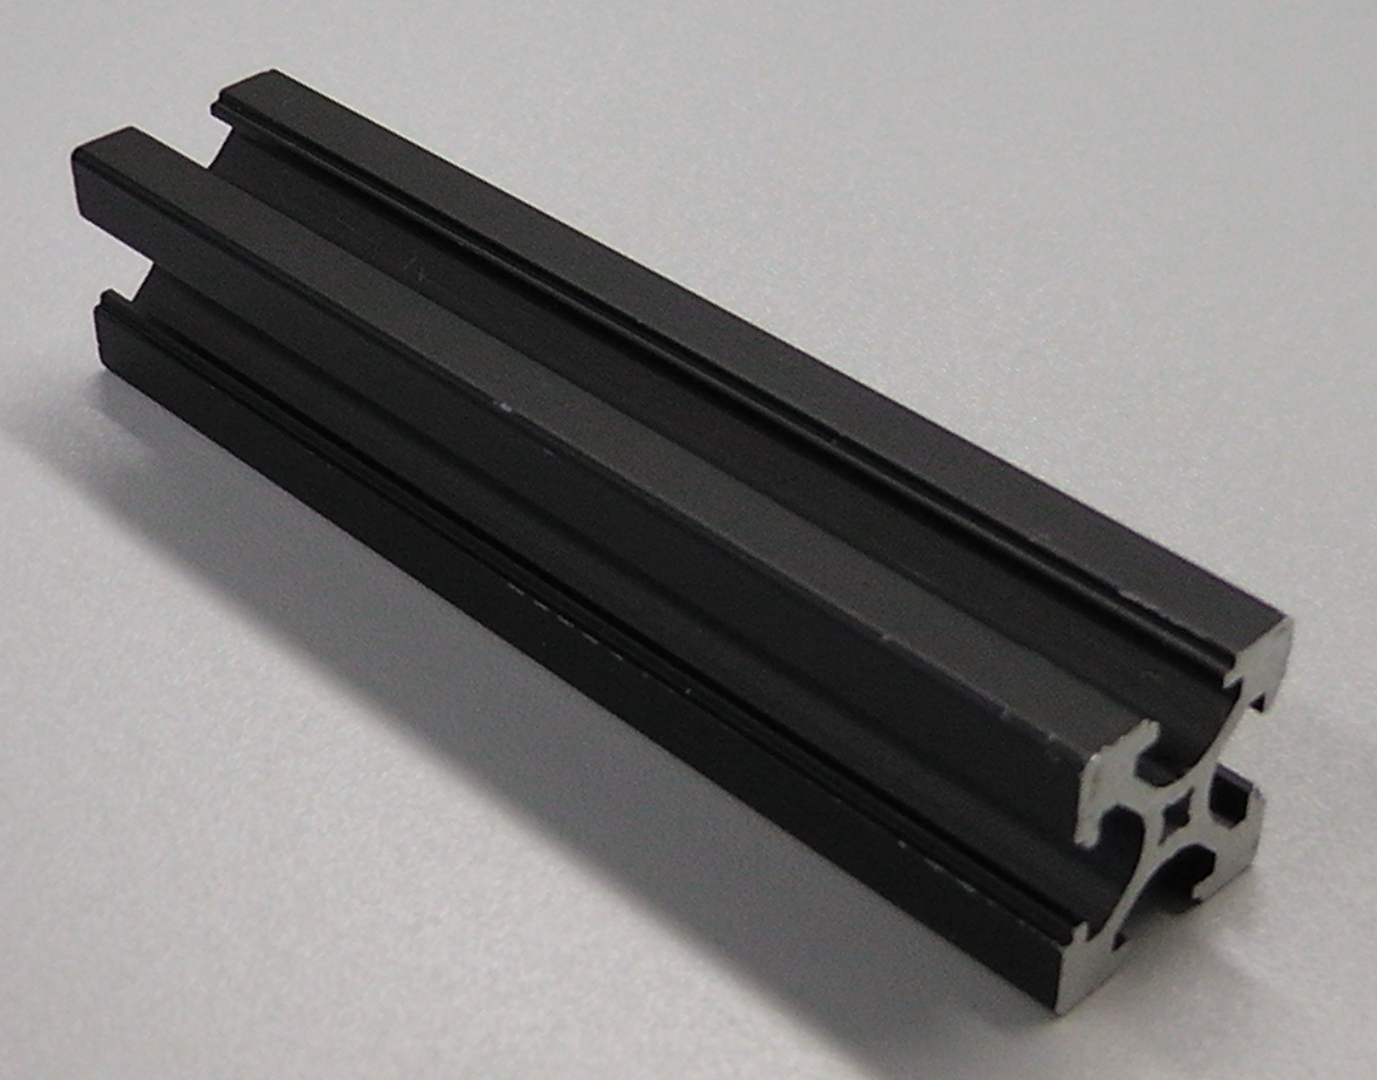
\includegraphics[width=.5\linewidth]{images/F20_20_B}
  			\caption{F20\_20\_B \cite{github_robocup@work}}
  			\label{fig:F20_20_B}
		\end{subfigure}
		\begin{subfigure}{.3\textwidth}
  			\centering
  			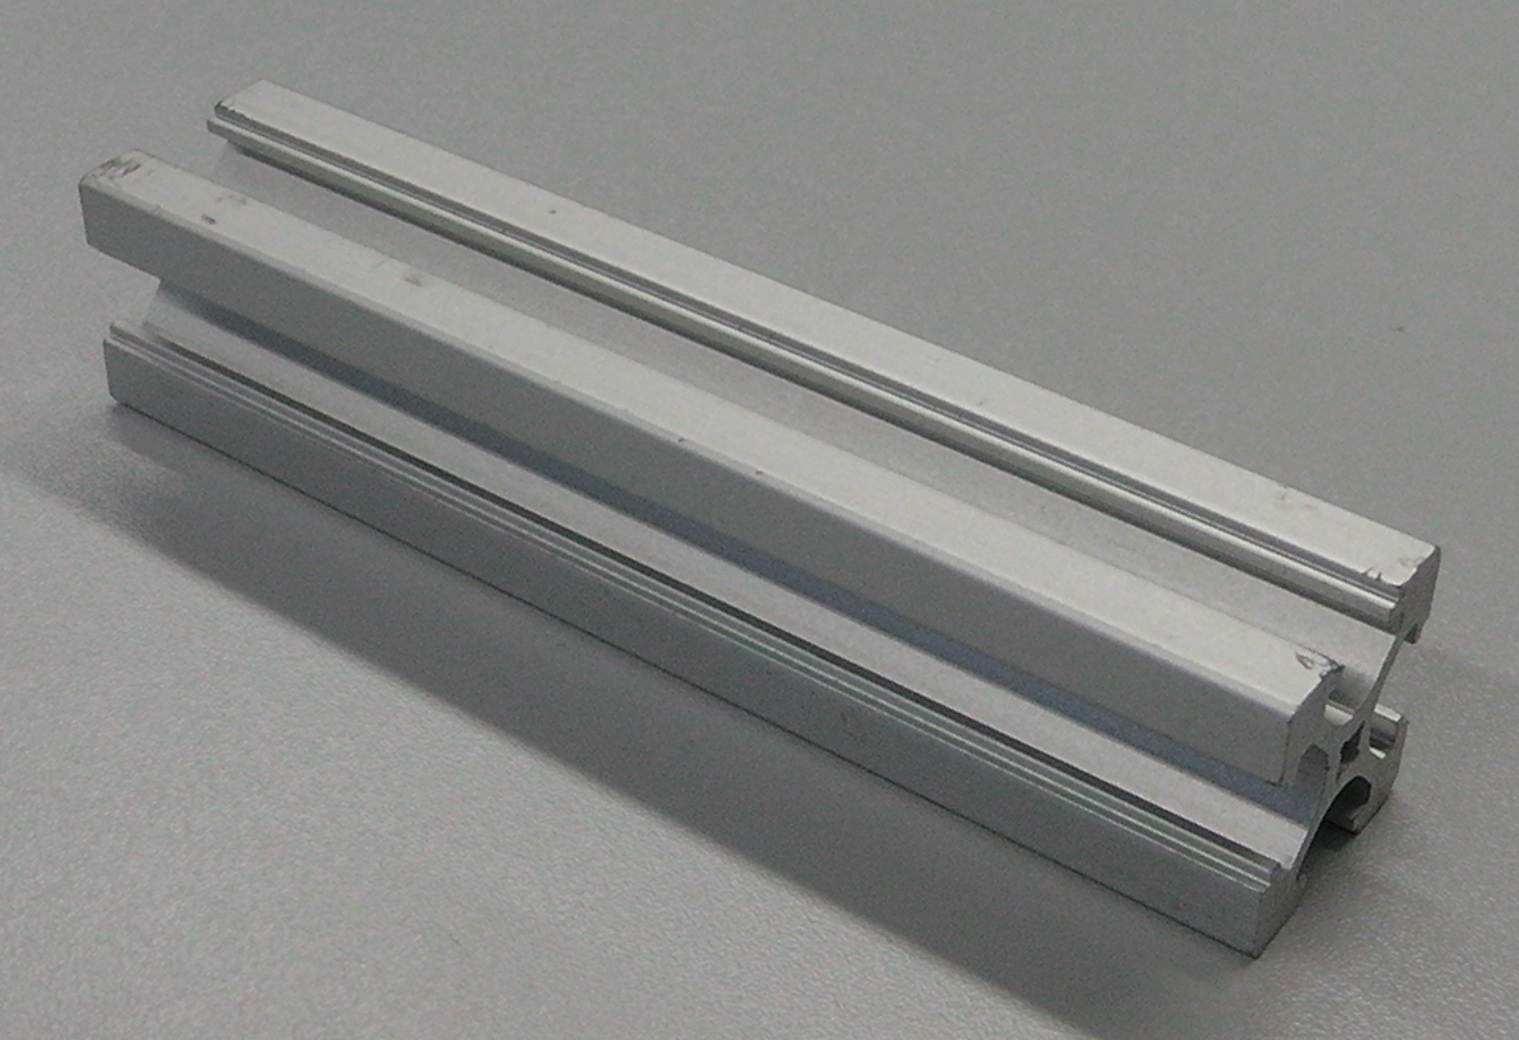
\includegraphics[width=.5\linewidth]{images/F20_20_G}
  			\caption{F20\_20\_G \cite{github_robocup@work}}
  			\label{fig:F20_20_G}
		\end{subfigure}\\
		\vspace{3mm}
		\begin{subfigure}{.3\textwidth}
  			\centering
  			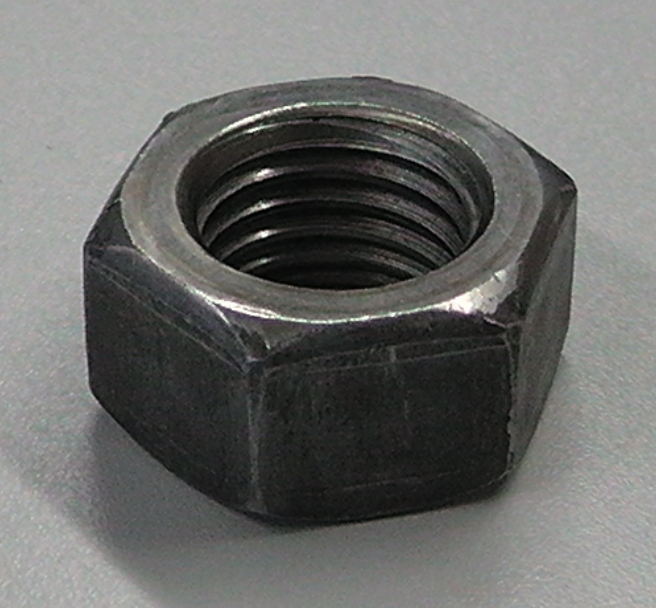
\includegraphics[width=.5\linewidth]{images/M20}
 			 \caption{M20 \cite{github_robocup@work}}
  			\label{fig:M20}
		\end{subfigure}
		\begin{subfigure}{.3\textwidth}
 			 \centering
  			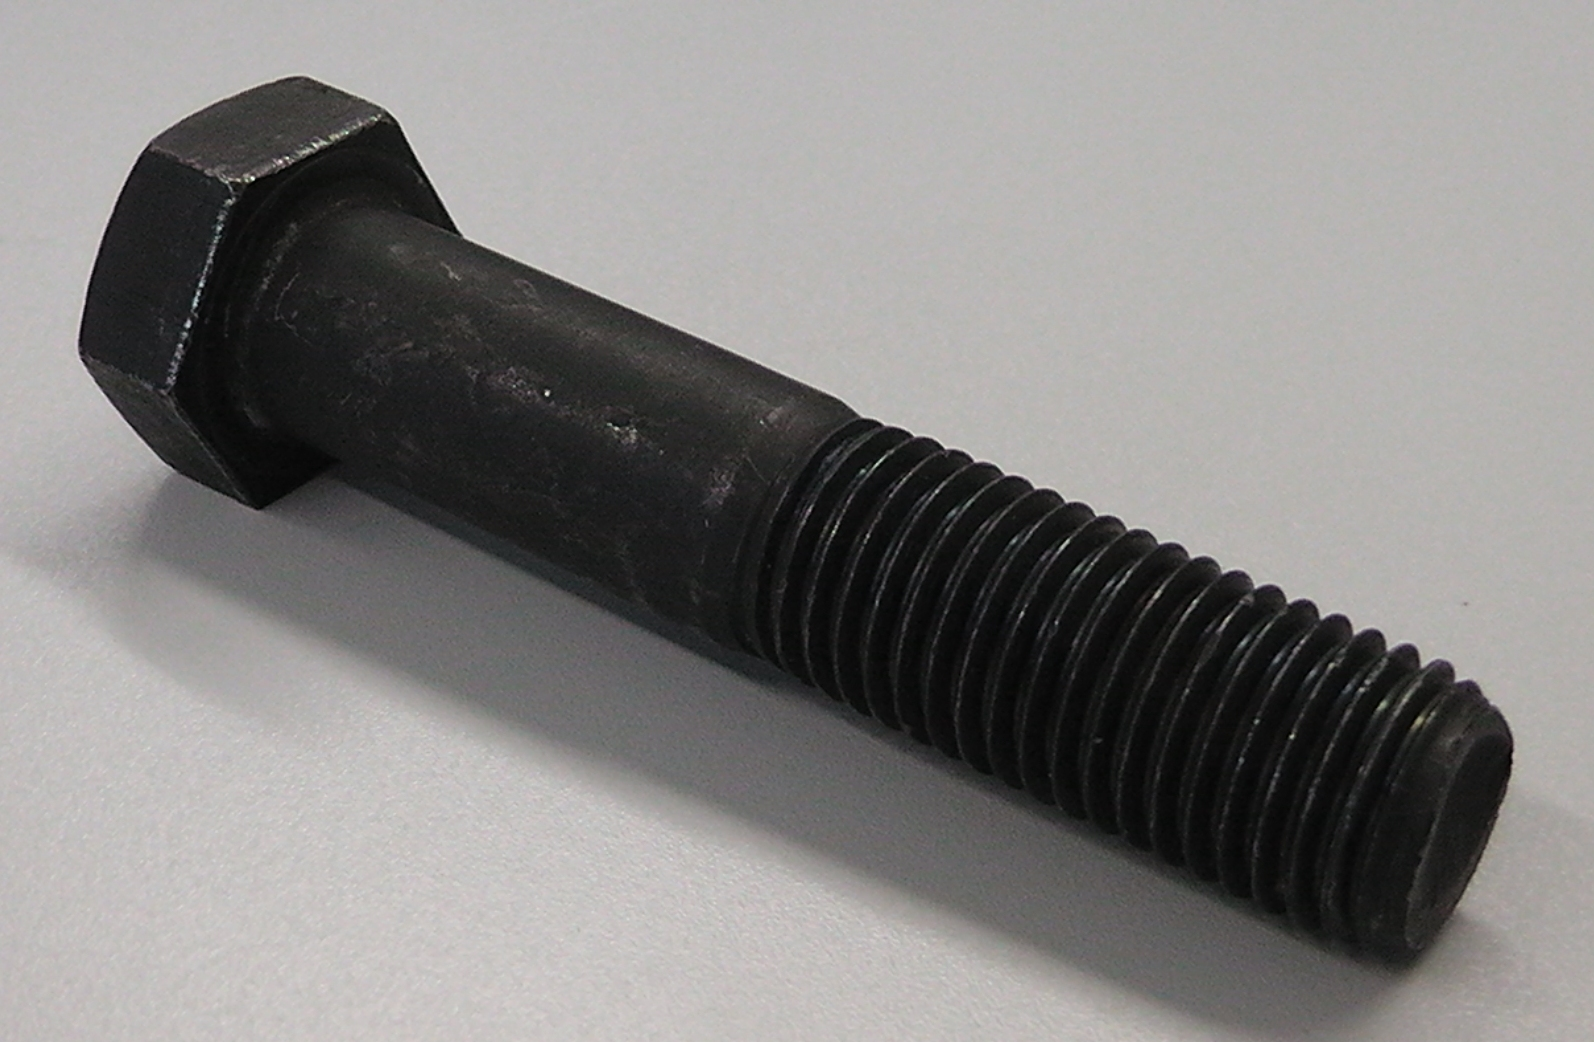
\includegraphics[width=.5\linewidth]{images/M20_100}
  			\caption{M20\_100 \cite{github_robocup@work}}
  			\label{fig:M20_100}
		\end{subfigure}
		\begin{subfigure}{.3\textwidth}
  			\centering
  			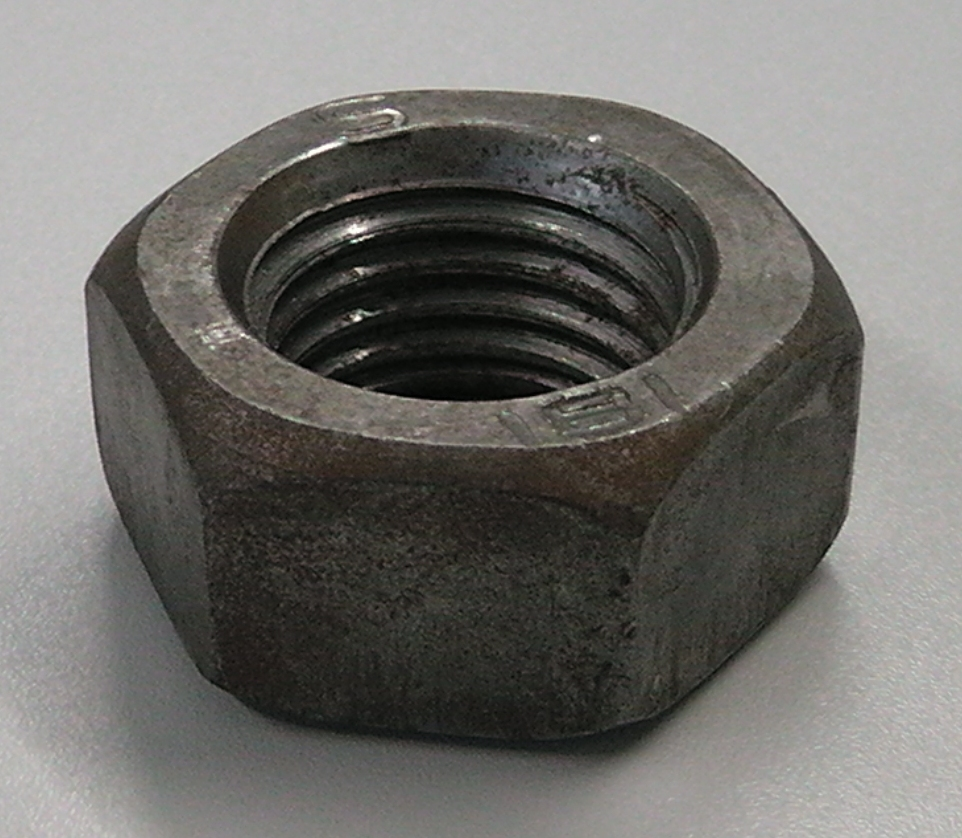
\includegraphics[width=.5\linewidth]{images/M30}
  			\caption{M30 \cite{github_robocup@work}}
  			\label{fig:M30}
		\end{subfigure}\\
		\vspace{3mm}
		\begin{subfigure}{.3\textwidth}
  			\centering
  			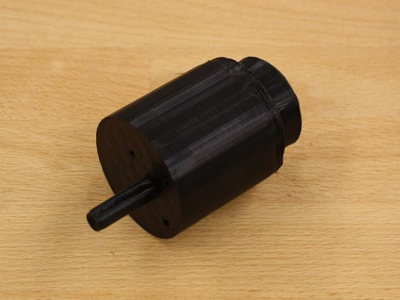
\includegraphics[width=.5\linewidth]{images/motor}
  			\caption{motor \cite{github_robocup@work}}
  			\label{fig:motor}
		\end{subfigure}
		\begin{subfigure}{.3\textwidth}
  			\centering
  			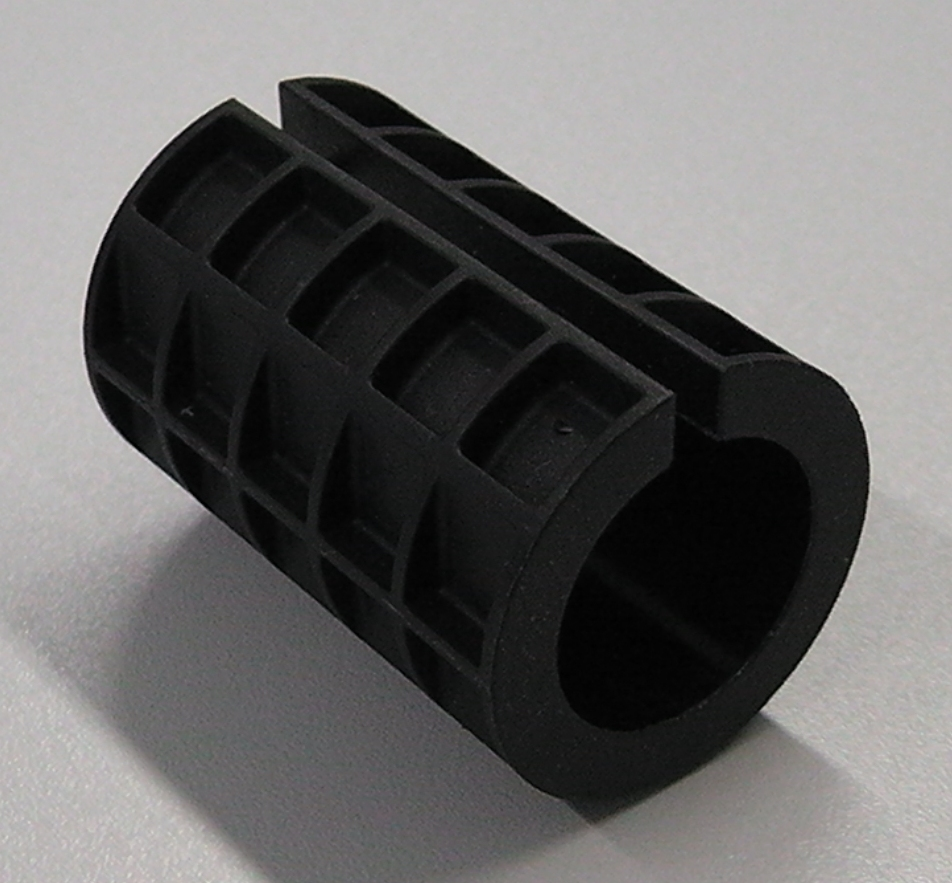
\includegraphics[width=.5\linewidth]{images/R20}
  			\caption{R20 \cite{github_robocup@work}}
  			\label{fig:R20}
		\end{subfigure}
		\begin{subfigure}{.3\textwidth}
  			\centering
  			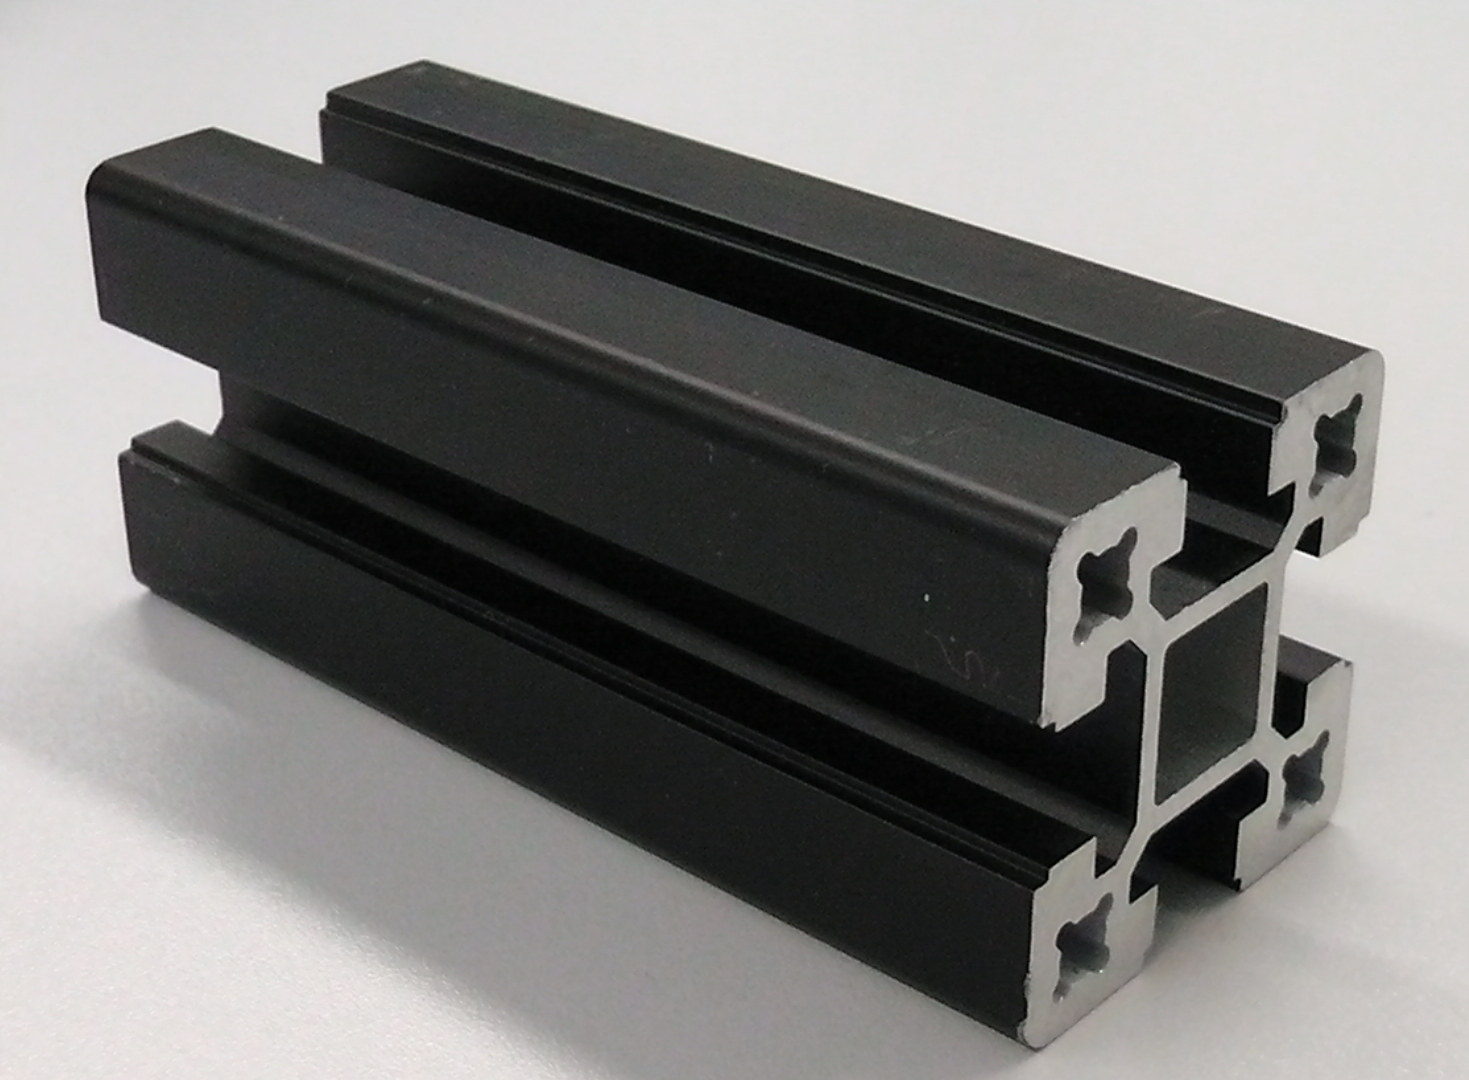
\includegraphics[width=.5\linewidth]{images/S40_40_B}
  			\caption{S40\_40\_B \cite{github_robocup@work}}
  			\label{fig:S40_40_B}
		\end{subfigure}\\
		\vspace{3mm}
		\begin{subfigure}{.3\textwidth}
  			\centering
  			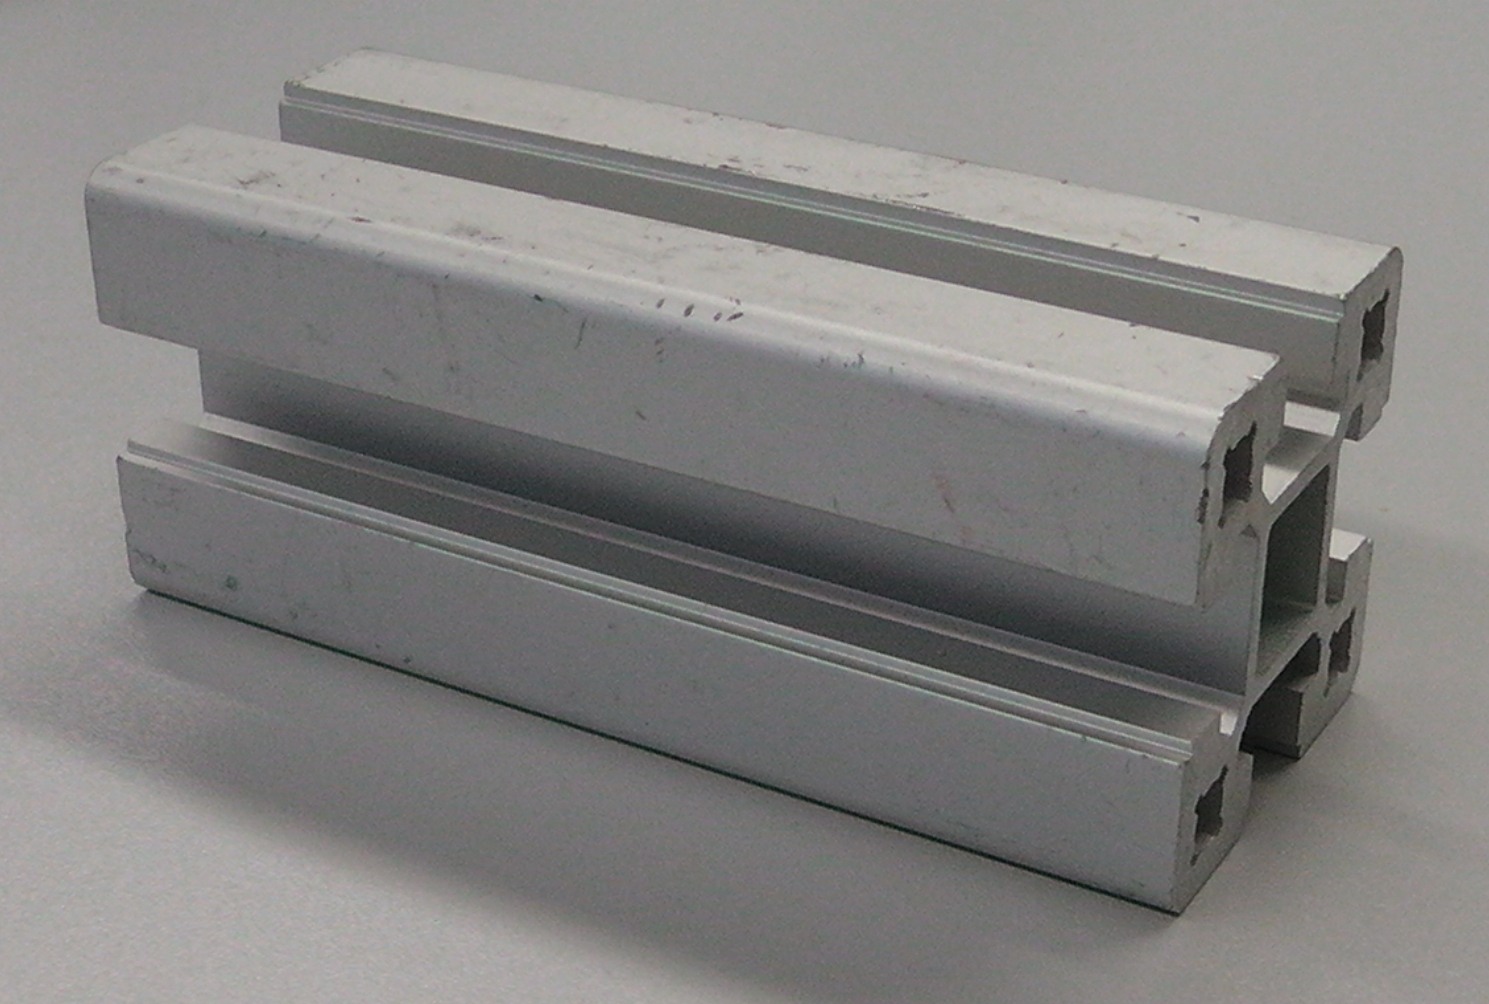
\includegraphics[width=.5\linewidth]{images/S40_40_G}
  			\caption{S40\_40\_G \cite{github_robocup@work}}
  			\label{fig:S40_40_G}
		\end{subfigure}
		\begin{subfigure}{.3\textwidth}
  			\centering
  			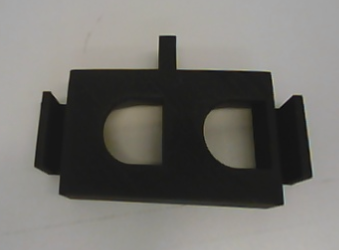
\includegraphics[width=.5\linewidth]{images/em_01}
  			\caption{em\_01}
  			\label{fig:em_01}
		\end{subfigure}
		\begin{subfigure}{.3\textwidth}
  			\centering
  			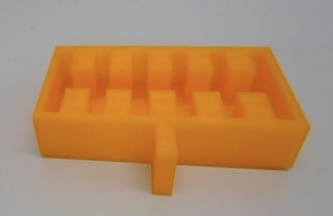
\includegraphics[width=.5\linewidth]{images/em_02}
  			\caption{em\_02}
  			\label{fig:em_02}
		\end{subfigure}
		\caption{Different objects required in the dataset}
		\label{Fig:objects}
	\end{figure}

Each of the objects were taken individually, placed on 3 different backgrounds and 30 images were taken. This lead to a total of 540 images which were to be manually labeled. Since, every pixel of the images needs to be labeled, the process of manual annotation would be time consuming. Therefore, a decision was made to first annotate the 540 images and later decide whether more images could be taken based on the effort required for annotation.

\section{Selection of a labeling tool}
In order to reduce the time required to annotate an image, it was imperative to select a tool which is specifically designed for semantic segmentation and also provides algorithms which helps the annotator by providing labeling automation to the highest possible extent.

The following available tools were evaluated for ease of use and time taken for annotation:
	\begin{itemize}
		\item LabelMe: web based tool is public and data would also be public.
		\item LabelMe Matlab toolbox: yet to try..
		\item University bonn annotation tool:
		\item Pixel annotation tool (using watershed algorithm): works in windows. Seems to be useful.
		\item Ratsnake: tool dint seem to be useful although the website had options like superpixel suggestions.
		\item LabelImg: Can be used but time consuming.
		\item Figi: used in medical image segmentation. Has many options. Still exploring.
		\item Supervisely.
		\item MATLAB ImageLabeler available in release R2017b (Computer Vision Toolbox).
	\end{itemize}

\section{Description of the labeling process}
\label{section:process}
MATLAB ImageLabeler was used for the labeling process. At first, label definitions are created and exported to a .mat file. This file is used to load label definitions for all images to maintain consistency of labels. The contents of the .mat file is shown in the Figure \ref{Fig:labeldef}.
	
	\begin{figure}
		\begin{subfigure}{.5\textwidth}
			\centering
			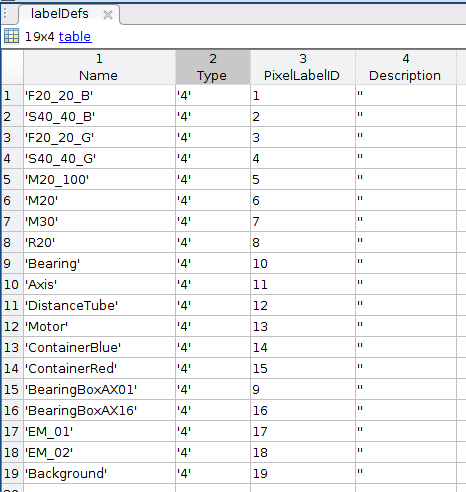
\includegraphics[width=1\linewidth]{images/labelDef}
			\caption{}
			\label{Fig:labeldef}
		\end{subfigure}
		\begin{subfigure}{.5\textwidth}
			\centering
			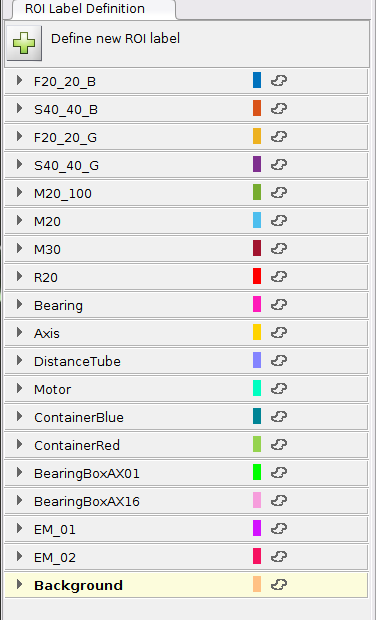
\includegraphics[width=0.83\linewidth]{images/roi_label_defintions}
			\caption{}
			\label{Fig:ROI}
		\end{subfigure}
		\caption{(a) Contents of the labelDefs .mat file, (b) ROI Label Definitions window.}
		\label{Fig:def_ROI}
	\end{figure}
	
The ImageLabeler app, by default, provides different tools which help create pixelwise labels. The tools are shown in the Figure \ref{Fig:IL_tools}. These tools become accessible once an image and the label definitions are loaded. A short description of the tools is given below:
	\begin{figure}
		\centering
		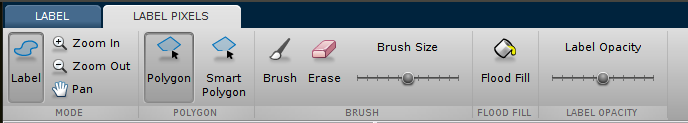
\includegraphics[scale=0.55]{images/label_tools}
		\caption{Tools provided by the ImageLabeler app}
		\label{Fig:IL_tools}
	\end{figure}
	
	\begin{itemize}
		\item Polygon: This can be used to trace an object boundary by placing dots. Once a closed contour is created, pixels within the contour get assigned the corresponding object label.
		\item Smart Polygon: Can be used in a similar fashion like the Polygon tool. This tool, in addition, tries to reach out to the nearby edges of the drawn polygon.
		\item Brush and Erase: Square shaped brush and eraser to either label a region or remove labels from a region. The size of the square can be changed by using the Brush Size slider.
		\item Flood Fill: This tool provides same labels to pixels which are similar in terms of the intensity with the selected pixel.
		\item Label Opacity: This tool provides a sliding bar which varies the opacity of the overlayed labels on the image. This is helpful to visualize the assigned labels.
		\item Zoom In, Zoom Out, Pan: These tools improve the ease of labeling by providing means to focus on particular regions by zooming and panning.
	\end{itemize}
	
The ImageLabeler app by default assigns different colors to different objects to aid visualization. The label colors are shown in the ROI Label Definition window shown in Figure \ref{Fig:ROI}. An example of an object in the ImageLabeler tool once the annotation is complete is shown in Figure \ref{Fig:ex_ann}.
	
	\begin{figure}
		\centering
		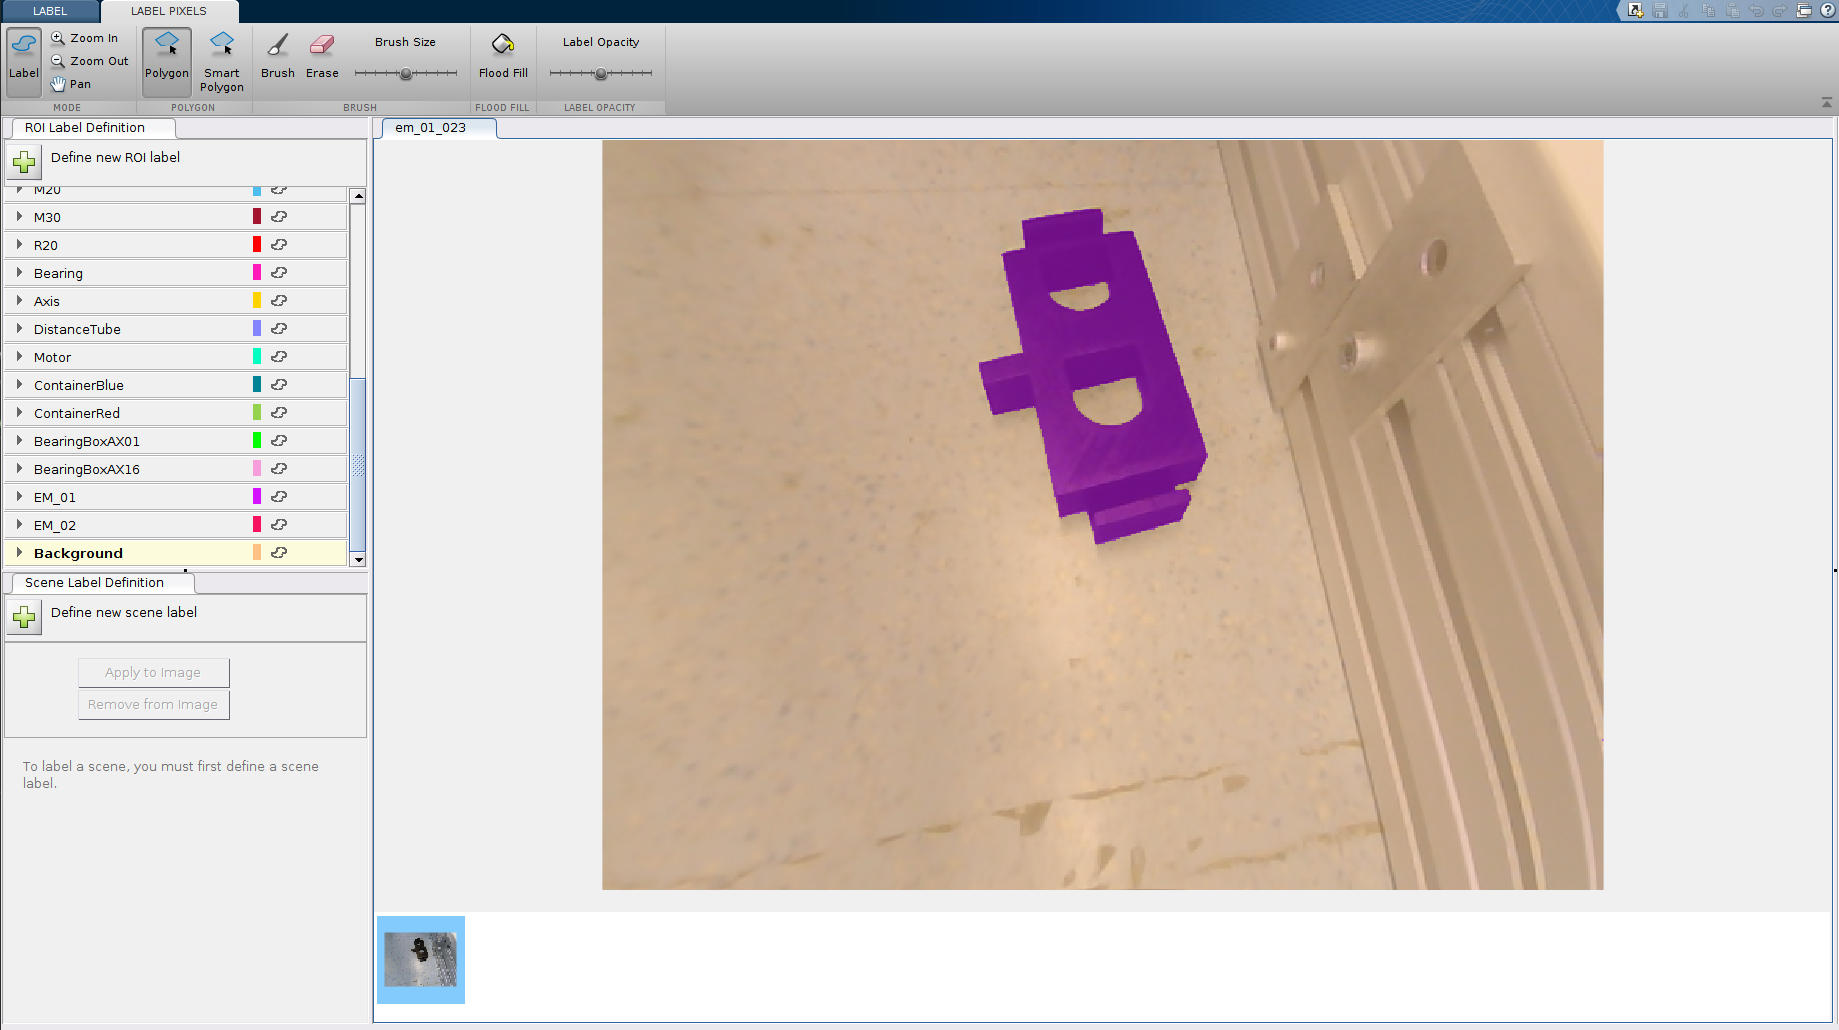
\includegraphics[scale=0.2]{images/imglabler_eg}
		\caption{An object labeled in the ImageLabeler.}
		\label{Fig:ex_ann}
	\end{figure}
	
The ImageLabeler app does not provide any tool to label all unlabeled pixels as background. In order to save time, the following workarounds have been used:
	\begin{itemize}
		\item The images taken for the dataset each have only one object in them.
		\item Only the object region is labeled.
		\item Since the ImageLabeler app does not provide any tool to label all unlabeled pixels as background, a python code which simply reads the label image and replaces unlabeled values 0 with background label value 19, was used for this purpose. The code is also used to double check the label image in order to avoid noisy labeling.
	\end{itemize}
	
The Export Labels --$>$ To File option can be used to save the annotations. This is done for all images individually to arrive at the folder structure shown in Figure \ref{Fig:fsa}.
	
The saved .mat file can be loaded into ImageLabeler again to further modify labels if required later. The 'Label\_1.png' file located in the PixelLabelData folder (as can be seen in Figure  \ref{Fig:fsa}) is the label image. This image is renamed to have the same name as the image file and a folder structure as in Figure  \ref{Fig:fsb} is created by using a python code.
	
\begin{center}
	\begin{figure}
		\begin{subfigure}{.5\textwidth}
			\centering
			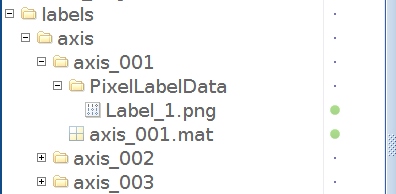
\includegraphics[width=1\linewidth]{images/folder_structure}
			\caption{Folder structure of saved labels}
			\label{Fig:fsa}
		\end{subfigure}
		\begin{subfigure}{.5\textwidth}
			\centering
			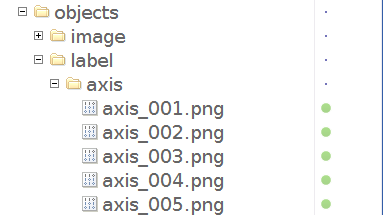
\includegraphics[width=1\linewidth]{images/folder_structure_aug}
			\caption{Rearranged folder structure}
			\label{Fig:fsb}
		\end{subfigure}
		\caption{Different folder structures}
		\label{Fig:fs}
	\end{figure}
\end{center}

The final folder structure is shown in Figure \ref{Fig:fsil}. The image folder and label folder are similar and contain object images and corresponding label images with same names.

\begin{center}
	\begin{figure}
		\begin{subfigure}{.5\textwidth}
			\centering
			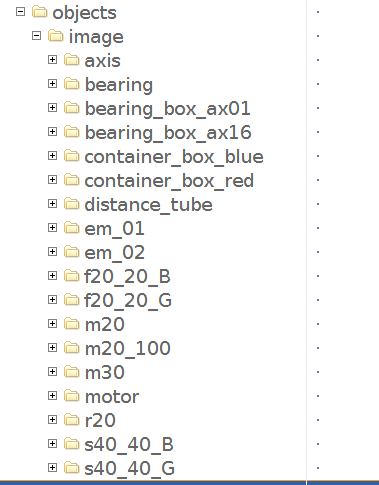
\includegraphics[width=1\linewidth]{images/folder_image}
			%\caption{}
			\label{Fig:fsila}
		\end{subfigure}
		\begin{subfigure}{.5\textwidth}
			\centering
			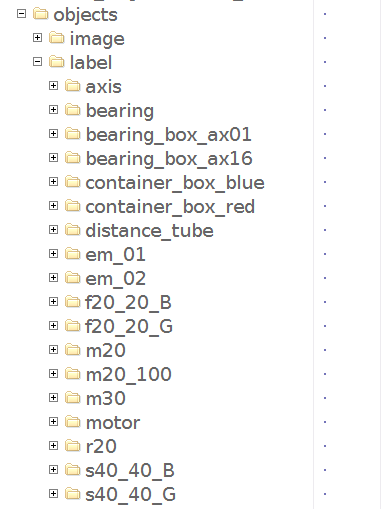
\includegraphics[width=1\linewidth]{images/folder_label}
			%\caption{}
			\label{Fig:fsilb}
		\end{subfigure}
		\caption{Folder structure showing different object folders in both image and label folders.}
		\label{Fig:fsil}
	\end{figure}
\end{center}

\section{Artificial image generation algorithm}

\subsection{Motivation}
	\begin{itemize}
		\item Manually labeling 540 images with the described process in Section \ref{section:process} takes roughly 2160 minutes (roughly 4 minutes per image). This is equivalent to around 4 working days. Hence, creating a large dataset with manual labeling is not feasible.
		\item Taking images in a variety of real world backgrounds is also time consuming.
		\item Labeling images with multiple objects would take an even longer time.
	\end{itemize}
	
These drawbacks could be overcome by randomly placing objects on a variety of different background images automatically using an algorithm.

\subsection{Process of artificial image generation}
The artificial image generation algorithm requires that every image provided must have just one object. The algorithm can be used in two modes named "Generate artificial images" and "Save visuals". The first mode can be used to generate artificial images and if required save visualizations of labels. The second mode can be used to just save visualizations. Under the first mode, the entire process can be divided into 7 broad steps:
	\begin{itemize}
		\item[1] \textbf{External interface}: An interface to obtain possible parameters to control the generation process. These parameters are obtaiend through argparse command line GUI and are called generator options.
		\item[2] \textbf{Get backgrounds and data}: Fetch all the backgrouds, images and corresponding labels from the provided respective background, image and label paths. First, all the images in the backgrounds path are read. Then, all available images in the label path is read and the corresponding image files in the provided image path is read. The images in the image path must have the same name as that of the corresponding labels but can be of a different format. The default image format is ".jpg".
		\item[3] \textbf{Get object details}: Fetch details regarding every object and its different scales. The details include information regarding object locations in an image, object values, label values, the object name, points in pixel space denoting a bounding rectangle around the object, and object area. The scales for every object is determined at random. Scaled objects which are too small or too big as determined by generator options are removed.
		\item[4] \textbf{Generate augmenter list}: Every element in the augmenter list denotes an artificial image and contains information including the chosen background image, the number of objects to place in the artificial image, which objects from the object details list are selected and locations in pixel space where the selected objects need to be placed. In this stage, elements which are cluttered with too many objects are removed as determined by the generator options.
		\item[5] \textbf{Generate artificial images}: Based on every element in the augmenter list, artificial images and corresponding labels are generated. Every element is taken one by one. The selected objects are placed on the selected background in the corresponding specified location, one by one. The resultant artificial image and semantic label is saved in the directory specified using generator options. Additionally, object detection labels, semantic masks and visualization previews can be saved by configuring generator options.
		\item[6] \textbf{Visualize results}: The generated images and labels are visualized to verify the generation process.
		\item[7] \textbf{Save results}: The obtained resultant artificial images, corresponding labels and generated visualizations are saved.
	\end{itemize}
	
Under the second mode, steps 3 to 6 in the above process is skipped. Step 2 fetches also the object detection labels in addition to the image and semantic labels. Step 7 saves the visualizations of read image, semantic labels and object detection labels.
		

\subsection{Generator options}

A number of arguments can be configured to control the generation process. Configuration of generator options is possible through command line GUI. Details regarding the arguments are provided in Table \ref{Table:godes} and in Table \ref{Table:govals}. 

\begin{table}
\centering
\begin{tabular}{|c|c|c|c|c|c|c|c|}
\hline 
\textbf{Generator options} & Description \\ 
\hline 
\textbf{mode} & \makecell{1: Generate artificial images; 2: Save visuals.} \\ 
\hline 
\textbf{image\_dimension} & \makecell{Dimension of the real images.} \\ 
\hline 
\textbf{num\_scales} & \makecell{Number of scales including original object scale.} \\ 
\hline 
\textbf{backgrounds\_path} & \makecell{Path to directory where the background images are located.} \\ 
\hline 
\textbf{image\_path} & \makecell{Path to directory where real images are located.} \\ 
\hline 
\textbf{label\_path} & \makecell{Path to directory where labels are located.} \\ 
\hline 
\textbf{obj\_det\_label\_path} & \makecell{Path to directory where the object detection \\csv labels are located.} \\ 
\hline 
\textbf{real\_img\_type} & \makecell{The format of the real image.} \\ 
\hline 
\textbf{min\_obj\_area} & \makecell{Minimum area in percentage allowed for \\an object in image space.} \\ 
\hline 
\textbf{max\_obj\_area} & \makecell{Maximum area in percentage allowed for \\an object in image space.} \\ 
\hline 
\textbf{save\_label\_preview} & \makecell{Save image+label in single image for preview.} \\ 
\hline 
\textbf{save\_obj\_det\_label} & \makecell{Save object detection labels in csv files.} \\ 
\hline  
\textbf{save\_mask} & \makecell{Save images showing the segmentation mask.} \\ 
\hline 
\textbf{save\_overlay} & \makecell{Save segmentation label overlaid on image.} \\ 
\hline 
\textbf{overlay\_opacity} & \makecell{Opacity of label on the overlaid image.} \\ 
\hline 
\textbf{image\_save\_path} & \makecell{Path where the generated artificial image needs\\ to be saved.} \\ 
\hline 
\textbf{label\_save\_path} & \makecell{Path where the generated segmentation label needs\\ to be saved.} \\ 
\hline 
\textbf{preview\_save\_path} & \makecell{Path where object detection labels needs to be saved.} \\ 
\hline 
\textbf{obj\_det\_save\_path} & \makecell{Path where object detection labels needs to be saved.} \\ 
\hline 
\textbf{mask\_save\_path} & \makecell{Path where segmentation masks needs to be saved.} \\ 
\hline 
\textbf{overlay\_save\_path} & \makecell{Path where overlaid images needs to be saved.} \\ 
\hline 
\textbf{start\_index} & \makecell{Index from which image and label names should start.} \\ 
\hline 
\textbf{name\_format} & \makecell{The format for image file names.} \\
\hline 
\textbf{remove\_clutter} & \makecell{Remove images cluttered with objects.} \\
\hline 
\textbf{num\_images} & \makecell{Number of artificial images to generate.} \\ 
\hline 
\textbf{max\_objects} & \makecell{Maximum number of objects allowed in an image.} \\ 
\hline 
\textbf{num\_regenerate} & \makecell{Number of regeneration attempts of removed details dict.} \\ 
\hline 
\textbf{min\_distance} & \makecell{Minimum pixel distance required between two objects.} \\ 
\hline 
\textbf{max\_occupied\_area} & \makecell{Maximum object occupancy area allowed.} \\ 
\hline 
\textbf{scale\_ranges} & \makecell{Can be used to change the zoom range of specific objects.} \\ 
\hline 
\end{tabular}
\caption{Description of generator options} 
\label{Table:godes}
\end{table}

\begin{table}
\centering
\begin{tabular}{|c|c|c|c|c|c|c|c|}
\hline 
\textbf{Generator options} & Default value & \makecell{Is required?} \\ 
\hline 
\textbf{mode} & \makecell{1} & \makecell{Not required} \\ 
\hline 
\textbf{image\_dimension} & \makecell{[480, 640]} & \makecell{Not required} \\ 
\hline 
\textbf{num\_scales} & \makecell{'randomize'} & \makecell{Not required} \\ 
\hline 
\textbf{backgrounds\_path} & \makecell{None} & \makecell{Required if mode is 1} \\ 
\hline 
\textbf{image\_path} & \makecell{-} & \makecell{Required} \\ 
\hline 
\textbf{label\_path} & \makecell{-} & \makecell{Required} \\ 
\hline 
\textbf{obj\_det\_label\_path} & \makecell{None} & \makecell{Required if save\_label\_preview \\is True and mode is 2} \\ 
\hline 
\textbf{real\_img\_type} & \makecell{'.jpg'} & \makecell{Not required} \\ 
\hline 
\textbf{min\_obj\_area} & \makecell{20} & \makecell{Not required} \\ 
\hline 
\textbf{max\_obj\_area} & \makecell{70} & \makecell{Not required} \\ 
\hline 
\textbf{save\_label\_preview} & \makecell{False} & \makecell{Not required} \\ 
\hline 
\textbf{save\_obj\_det\_label} & \makecell{False} & \makecell{Not required} \\ 
\hline  
\textbf{save\_mask} & \makecell{False} & \makecell{Not required} \\ 
\hline 
\textbf{save\_overlay} & \makecell{False} & \makecell{Not required} \\ 
\hline 
\textbf{overlay\_opacity} & \makecell{0.6} & \makecell{Not required} \\ 
\hline 
\textbf{image\_save\_path} & \makecell{None} & \makecell{Required if \\mode is 1} \\ 
\hline 
\textbf{label\_save\_path} & \makecell{None} & \makecell{Required if \\mode is 1} \\ 
\hline 
\textbf{preview\_save\_path} & \makecell{None} & \makecell{Required if \\save\_label\_preview is True} \\ 
\hline 
\textbf{obj\_det\_save\_path} & \makecell{None} & \makecell{Required if \\save\_obj\_det\_label is True} \\ 
\hline 
\textbf{mask\_save\_path} & \makecell{None} & \makecell{Required if \\save\_mask is True} \\ 
\hline 
\textbf{overlay\_save\_path} & \makecell{None} & \makecell{Required if \\save\_overlay is True} \\ 
\hline 
\textbf{start\_index} & \makecell{0 if mode is 1 \\ '' if mode is 2} & \makecell{Not required} \\ 
\hline 
\textbf{name\_format} & \makecell{'\%05d'} & \makecell{Not required} \\
\hline 
\textbf{remove\_clutter} & \makecell{True} & \makecell{Not required} \\
\hline 
\textbf{num\_images} & \makecell{20} & \makecell{Not required} \\ 
\hline 
\textbf{max\_objects} & \makecell{10} & \makecell{Not required} \\ 
\hline 
\textbf{num\_regenerate} & \makecell{100} & \makecell{Not required} \\ 
\hline 
\textbf{min\_distance} & \makecell{100} & \makecell{Not required} \\ 
\hline 
\textbf{max\_occupied\_area} & \makecell{0.8} & \makecell{Not required} \\ 
\hline 
\textbf{scale\_ranges} & \makecell{None} & \makecell{Not required} \\ 
\hline 
\end{tabular}
\caption{Default value of generator options and whether the options are required to be set.}
\label{Table:govals}
\end{table}

\subsection{Sample results}
Sample results of the artificial image generation algorithm can be seen in Figure \ref{Fig:sample}. These images are generated using different backgrounds and hence the dataset is referred to as variety of backgrounds dataset. The bounding box in the label visualization image represents the object detection label and the different colors of the segmentation labels denote different label values. The colors were chosen in such a way that they are as distinct from each other as possible \cite{simple_colors}.

	\begin{figure}
		\centering
		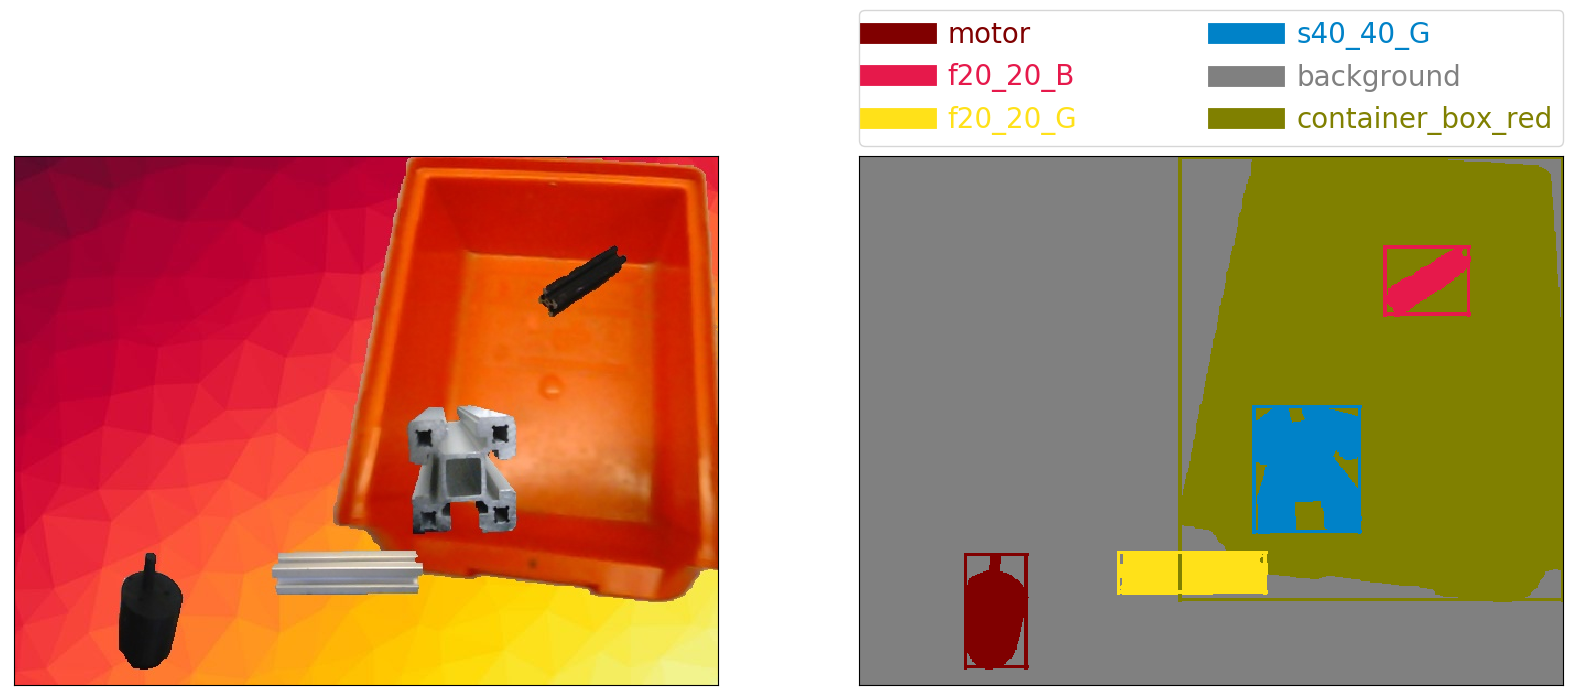
\includegraphics[scale=0.3]{images/sample_result_1}
		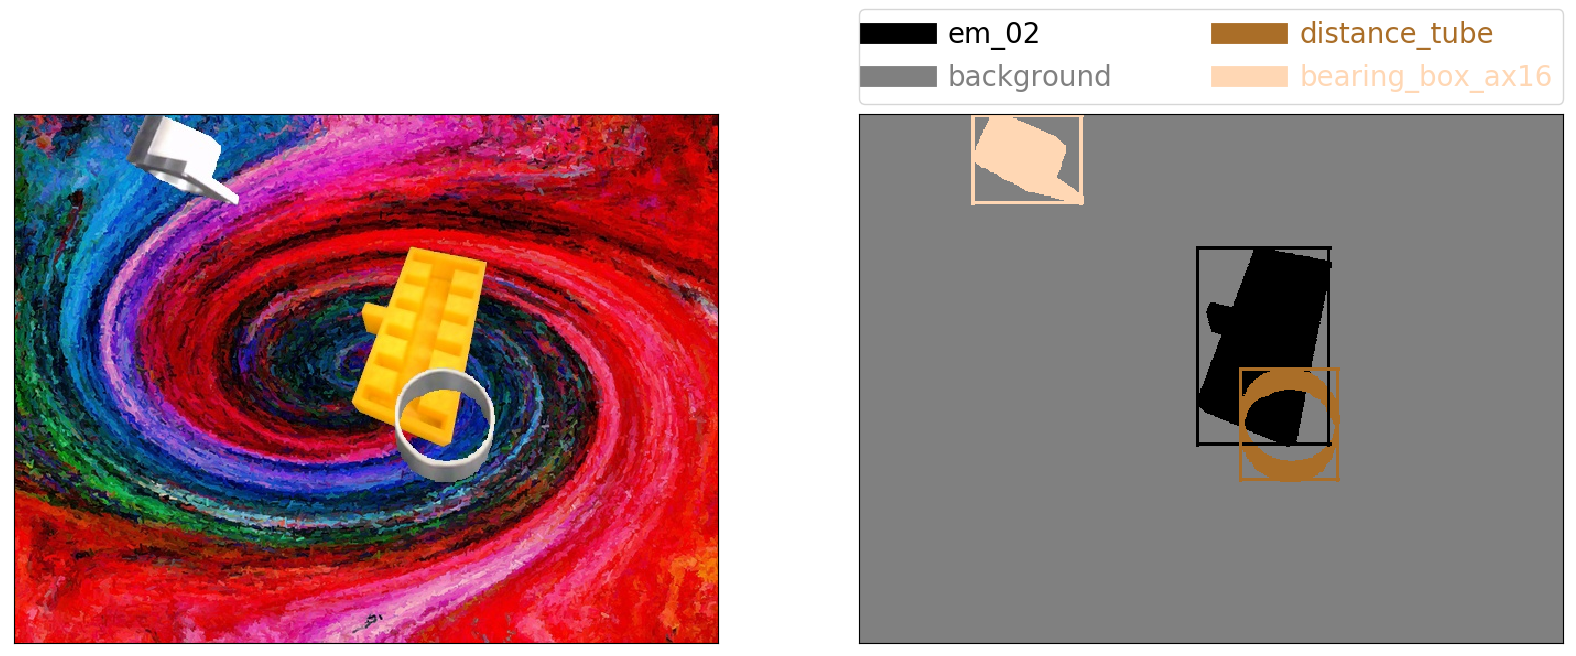
\includegraphics[scale=0.3]{images/sample_result_2}
		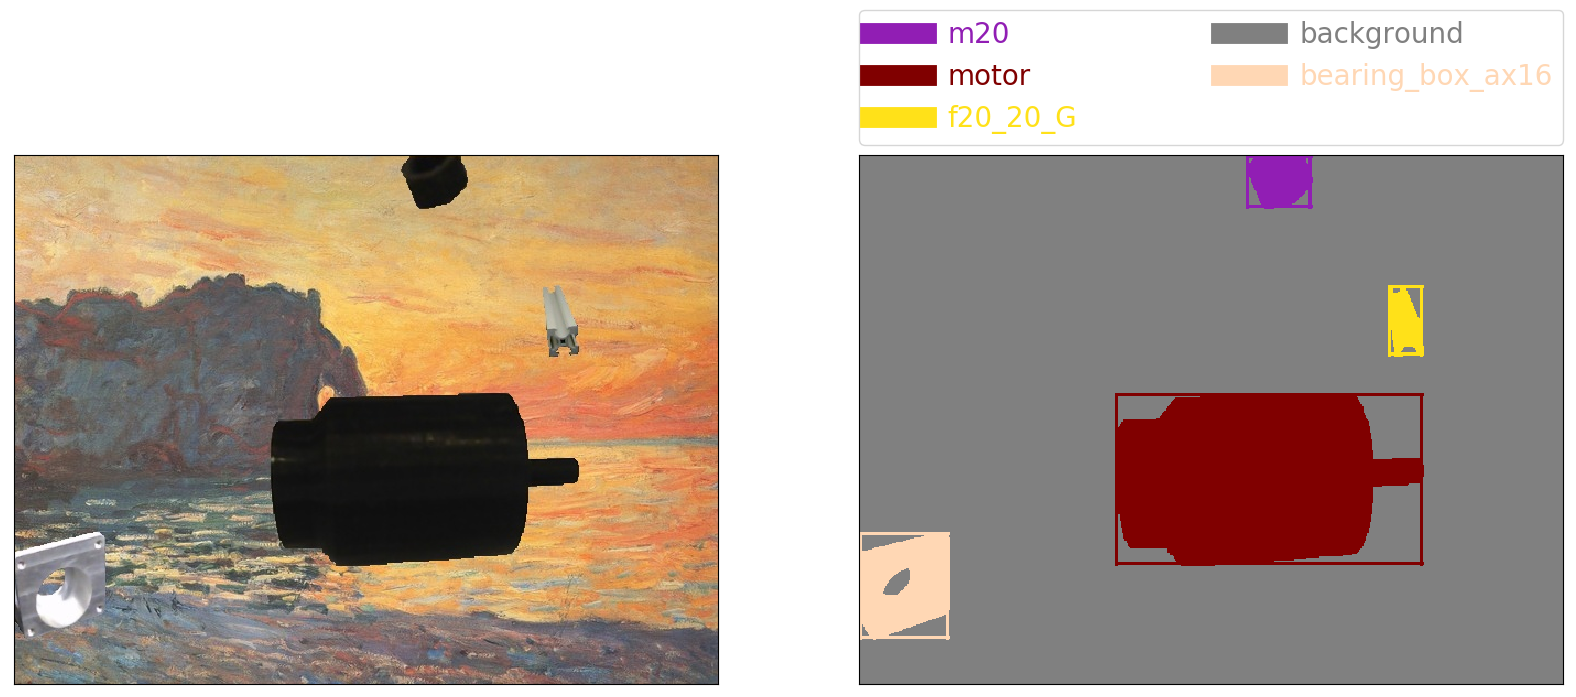
\includegraphics[scale=0.3]{images/sample_result_3}
		\caption{Sample results produced by the artificial image generation algorithm for the variety of backgronds dataset. In each row, the image on the left shows the generated artificial image and the image on the right shows a visualization of the semantic segmentation label and object detection label. At the top of every label visualization image, the objects in the image and their corresponding colors in the visualization are indicated.}
		\label{Fig:sample}
	\end{figure}
	
\subsection{Downloading background images}
Different background images were used for the artificial image generation process. Since a large number of backgrounds were required, manual download was time consuming. Hence, the "google-images-download" \cite{image_downloader} script was used to auto download images. The search keywords used to obtain the background images are listed in Table \ref{Table:download}. From the downloaded images, the required number of images for each dataset split were selected. For the white backgrounds dataset, many different search keywords were tried as is evident from the Table  \ref{Table:download}. This was because many of the downloaded images did not contain sufficient white regions. Images which were not of the dimensions used in the dataset (480$\times$640) were rescaled.

\begin{table}
	\centering
	\begin{tabular}{|c|c|c|c|c|c|c|c|}
	\hline 
    Used in & Search keyword(s) & \makecell{Number of \\images selected} \\ 
	\hline 
	Training set & \makecell{640x480 background images, \\640x480 textures images, \\640x480 wallpapers} & 150 \\ 
	\hline 
	Validation set & 640x480 abstract & 25 \\ 
	\hline 
	Test set & 640x480 paintings & 25 \\ 
	\hline 
	Shades of white & \makecell{640x480 white abstract, \\640x480 white backgrounds, \\640x480 white textures, \\640x480 white wallpaper, \\light gray, white, white clouds, \\white floors, white frost, white mist, \\white pebbles, white snow, \\white table textures} & 150 \\ 
	\hline 
	\end{tabular}
	\caption{This table lists the keywords used to download images used as background for artificial image generation.} 
	\label{Table:download}
\end{table}

	
\subsection{Notable features of the artificial image generator}

In this section, certain features of the artificial image generator which are noteworthy are listed.
	\begin{itemize}
		\item The generator automatically creates object detection labels in addition to semantic labels. The object detection labels are obtained by finding the rectangle points which describe a bounding rectangle around the semantic labels.
		\item The generated artificial images and labels can be visualized in three different ways. A preview which shows the image alongside the generated labels. A mask image showing the different classes in different colors. An overlay image in which the generated labels are overlayed on top of the corresponding generated images. The opacity of overlay can be configured through generator options. Examples of visualizations can be seen in Figure \ref{Fig:visuals} and in Figure \ref{Fig:sample}.
		
		\begin{figure}
			\centering
			\begin{subfigure}{.3\textwidth}
  				\centering
  				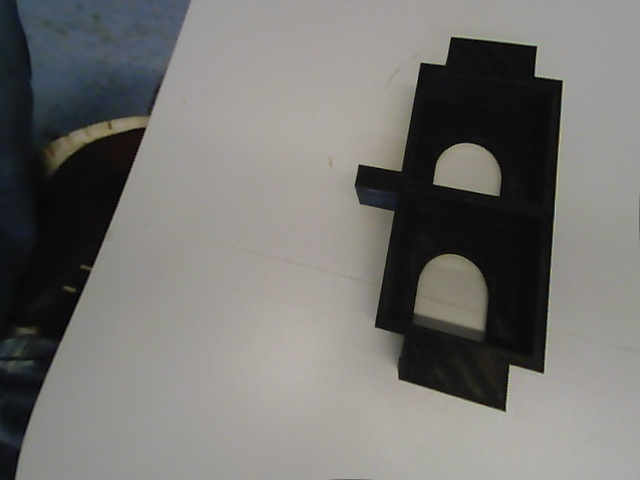
\includegraphics[width=.9\linewidth]{images/eg_image}
  				\caption{Image containing \\object em\_01}
  				\label{Fig:visualsa}
			\end{subfigure}%
			\begin{subfigure}{.3\textwidth}
  				\centering
  				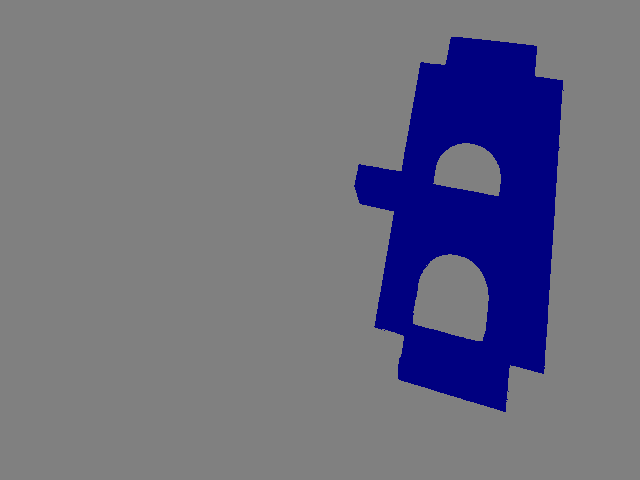
\includegraphics[width=.9\linewidth]{images/eg_mask}
  				\caption{Corresponding \\segmentation mask}
  				\label{Fig:visualsb}
			\end{subfigure}%
			\begin{subfigure}{.3\textwidth}
  				\centering
  				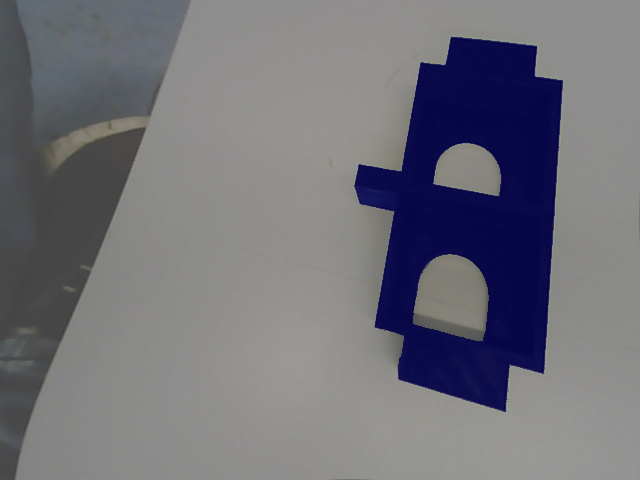
\includegraphics[width=.9\linewidth]{images/eg_overlay}
  				\caption{Corresponding overlay visualization}
  				\label{Fig:visualsc}
			\end{subfigure}%
		\caption{This figure shows examples of two different types of visualization, "mask" and "overlay". The third type "preview" can be seen in figure \ref{Fig:sample}}
		\label{Fig:visuals}
		\end{figure}
		
	\end{itemize}
	
\subsection{Artificial images for each dataset split}

The real images are split into training, validation and test sets. Real images in each of these sets are used to generate artificial images for the coresponding set. This ensures that the final training, validation and test sets are different from each other. The default scale range of [0.24, 1.2] is retained for all objects except for the "distance\_tube". The scale range of "distance\_tube" was set to [1.1, 2.0] for generating training artificial images and to [0.6, 1.2] for generating validation and test artificial images. This is because the lower limit of 0.24 in the default scale range zooms down "distance\_tube" in a manner that it is no longer perceivable which is not desired.

\section{Creation of dataset variants}
Different variants of the dataset are created based on the properties of the objects in the dataset, and the type of  background images used for generation of artificial images.
	\subsection{Motivation}
		Looking into the objects present in the dataset, it is apparent that some objects are similar in certain aspects. For instance, the objects m20 and m30 are very similar to each other except that m30 is bigger in size and has a slightly different color. Because of the similarities existing among objects, the segmentation model could face certain difficulties as listed below:
		\begin{itemize}
			\item \textbf{Inability to distinguish size}: The segmentation model is given no information regarding the positions of the camera or the object in the real world. If camera extrinsic calibration information is available to the segmentation model, the model could possibly learn to distinguish different sizes. However, such information is not available. In addition, the objects in the artificial images are randomly scaled to different sizes thereby removing any size related information available.
			\item \textbf{Inability to distinguish subtle variations in color}: The real images were taken under different lighting conditions. As a result, there is no consistent difference in color information available between classes. This makes it difficult for the segmentation model to learn patterns in color information.
			\item \textbf{Inability to distinguish shapes}: Certain objects are closly related to each other in terms of shape and differ only slightly. For instance, bearing\_box\_ax16 and bearing\_box\_ax01 are similar in shape except in a few viewpoints as illustrated in Figure \ref{Fig:sim1} and in Figure \ref{Fig:sim2}. In such cases, in certain viewpoints, the segmentation model would not be able to distinguish between similarly shaped objects.
			
\begin{figure}
	\centering
	\begin{subfigure}{.3\textwidth}
  		\centering
  		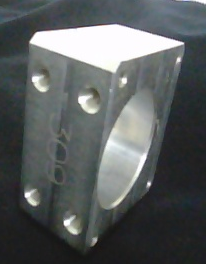
\includegraphics[width=.5\linewidth]{images/ax01_diff}
  		\caption{A viewpoint of \\bearing box ax01}
  		\label{Fig:sim1a}
	\end{subfigure}%
	\begin{subfigure}{.3\textwidth}
  		\centering
  		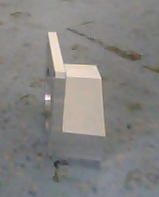
\includegraphics[width=.5\linewidth]{images/ax16_diff}
  		\caption{A viewpoint of \\bearing box ax16}
  		\label{Fig:sim1b}
	\end{subfigure}%
	\caption{A similar viewpoint of bearing box ax01 and bearing box ax16 where the difference in shapes between the two objects is clearly visible.}
	\label{Fig:sim1}
\end{figure}

\begin{figure}
	\centering
	\begin{subfigure}{.3\textwidth}
  		\centering
  		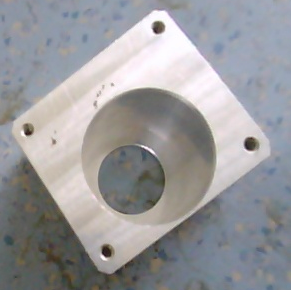
\includegraphics[width=.5\linewidth]{images/ax01_similar}
  		\caption{A viewpoint of \\bearing box ax01}
  		\label{Fig:sim2a}
	\end{subfigure}%
	\begin{subfigure}{.3\textwidth}
  		\centering
  		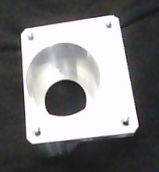
\includegraphics[width=.5\linewidth]{images/ax16_similar}
  		\caption{A viewpoint of \\bearing box ax16}
  		\label{Fig:sim2b}
	\end{subfigure}%
	\caption{A similar viewpoint of bearing box ax01 and bearing box ax16 where they appear similar in shape.}
	\label{Fig:sim2}
\end{figure}	
	\end{itemize}
	
	\subsection{Dataset variants}
	
	Four different dataset variants have been created as listed below:
	\begin{itemize}
		\item \textbf{atWork\_full}: This variant has different label values for all the 18 objects in the dataset and an additional label value for background. The total number of classes is 19 including background and the label values range from 0 to 18. The different classes in this variant along with their label values are listed in Table \ref{Table:variants}.
		\item \textbf{atWork\_size\_invariant}: In this variant, objects which are similar to each other in terms of shape but differ in size are combined together into one class. On this regard, f20\_20\_B and s40\_40\_B are combined and named f\_s20\_40\_20\_40\_B. Similarly, f20\_20\_G and s40\_40\_G are combined and named f\_s20\_40\_20\_40\_G. m20 and m30 are combined and named m20\_30. The two bearing boxes, bearing\_box\_ax01 and bearing\_box\_ax16 are also combined together as they are similar to each other in certain viewpoints. They form the new class bearing\_box. The objects in this variant along with their label values are listed in Table \ref{Table:variants}. This variant is named "atWork\_size\_invariant" as in this variant, the major change deals with the ignorance of the size of the objects as distinguishing information.
		\item \textbf{atWork\_similar\_shapes}: In the previous variant "atWork\_size\_invariant", objects similar in terms of shape but different in terms of color were treated as separate classes. In this variant, variation in terms of color is also ignored. In addition to the previous variant, f\_s20\_40\_20\_40\_B and f\_s20\_40\_20\_40\_G are combined and named f\_s20\_40\_20\_40\_B\_G. The container boxes, container\_box\_red and container\_box\_blue were also combined to form the new class container\_box. This variant is named "atWork\_similar\_shapes" as objects with similar shapes are given equal label values. Details regarding this variant are listed in Table \ref{Table:variants}.
		\item \textbf{atWork\_binary}: An interesting question would be, "how would a segmentation model perform when it is just tasked with segmenting foreground from background". To address this question, an additional variant is created called "atWork\_binary" where are the objects of interest are combined to form the "foreground" class with label value 1. The "background" class retains its label value of 0. The classes in this variant are listed in Table \ref{Table:variants}.
		
		\begin{table}
			\centering
			\begin{tabular}{|c|c|c|c|c|c|c|c|}
			\hline 
  			\makecell{Label \\Value} & \makecell{atWork\_\\full \\ objects} & \makecell{atWork\_size\_\\invariant \\ objects} & \makecell{atWork\_similar\_\\shapes \\ objects} & \makecell{atWork\_\\binary \\ objects} \\ 
			\hline
			0 & background & background & background & background \\ 
			\hline
			1 & f20\_20\_B & f\_s20\_40\_20\_40\_B & f\_s20\_40\_20\_40\_B\_G & foreground \\ 
			\hline
			2 & s40\_40\_B & f\_s20\_40\_20\_40\_G & m20\_100 & - \\ 
			\hline
			3 & f20\_20\_G & m20\_100 & m20\_30 & - \\ 
			\hline
			4 & s40\_40\_G & m20\_30 & r20 & - \\ 
			\hline
			5 & m20\_100 & r20 & bearing\_box & - \\ 
			\hline
			6 & m20 & bearing\_box & bearing & - \\ 
			\hline
			7 & m30 & bearing & axis & - \\ 
			\hline
			8 & r20 & axis & distance\_tube & - \\ 
			\hline	
			9 & bearing\_box\_ax01 & distance\_tube & motor & - \\ 
			\hline		
			10 & bearing & motor & container & - \\ 
			\hline
			11 & axis & container\_box\_blue & em\_01 & - \\ 
			\hline
			12 & distance\_tube & container\_box\_red & em\_02 & - \\ 
			\hline
			13 & motor & em\_01 & - & - \\ 
			\hline
			14 & container\_box\_blue & em\_02 & - & - \\ 
			\hline
			15 & container\_box\_red & - & - & - \\ 
			\hline
			16 & bearing\_box\_ax16 & - & - & - \\ 
			\hline
			17 & em\_01 & - & - & - \\ 
			\hline
			18 & em\_02 & - & - & - \\ 
			\hline
			\end{tabular}
			\caption{This table lists the objects in each variant and its corresponding label value.} 
			\label{Table:variants}
		\end{table}
		
	\end{itemize}

	\subsection{White backgrounds dataset}
The backgrounds used for the artificial image generation process are images with a variety of different colors, textures and so on. In essense, the background images do not seem to follow any pattern as such. As a result, the generated artificial images are unlikely to be similar to an image taken by an atWork robot. In order to address this, the background images used in the artificial image generation process are all replaced with images which mostly contain shades of white color in them. With this as the only change, the entire artificial image generation process and variant creation process is repeated to arrive at a new dataset which is named "white backgrounds dataset". Sample visualizations of artificial images generated for this dataset can be seen in Figure \ref{Fig:samplewhite}.

	\begin{figure}
		\centering
		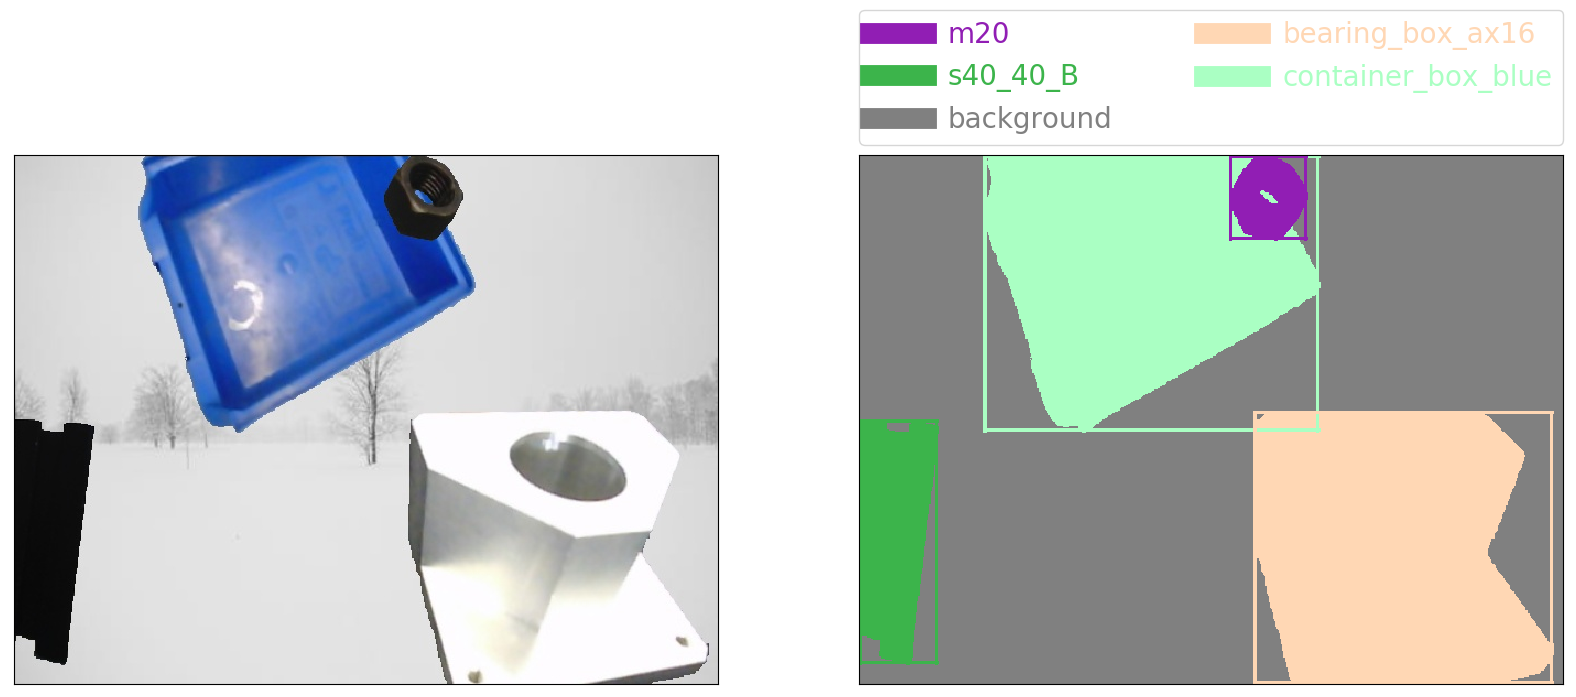
\includegraphics[scale=0.3]{images/sample_white_1}
		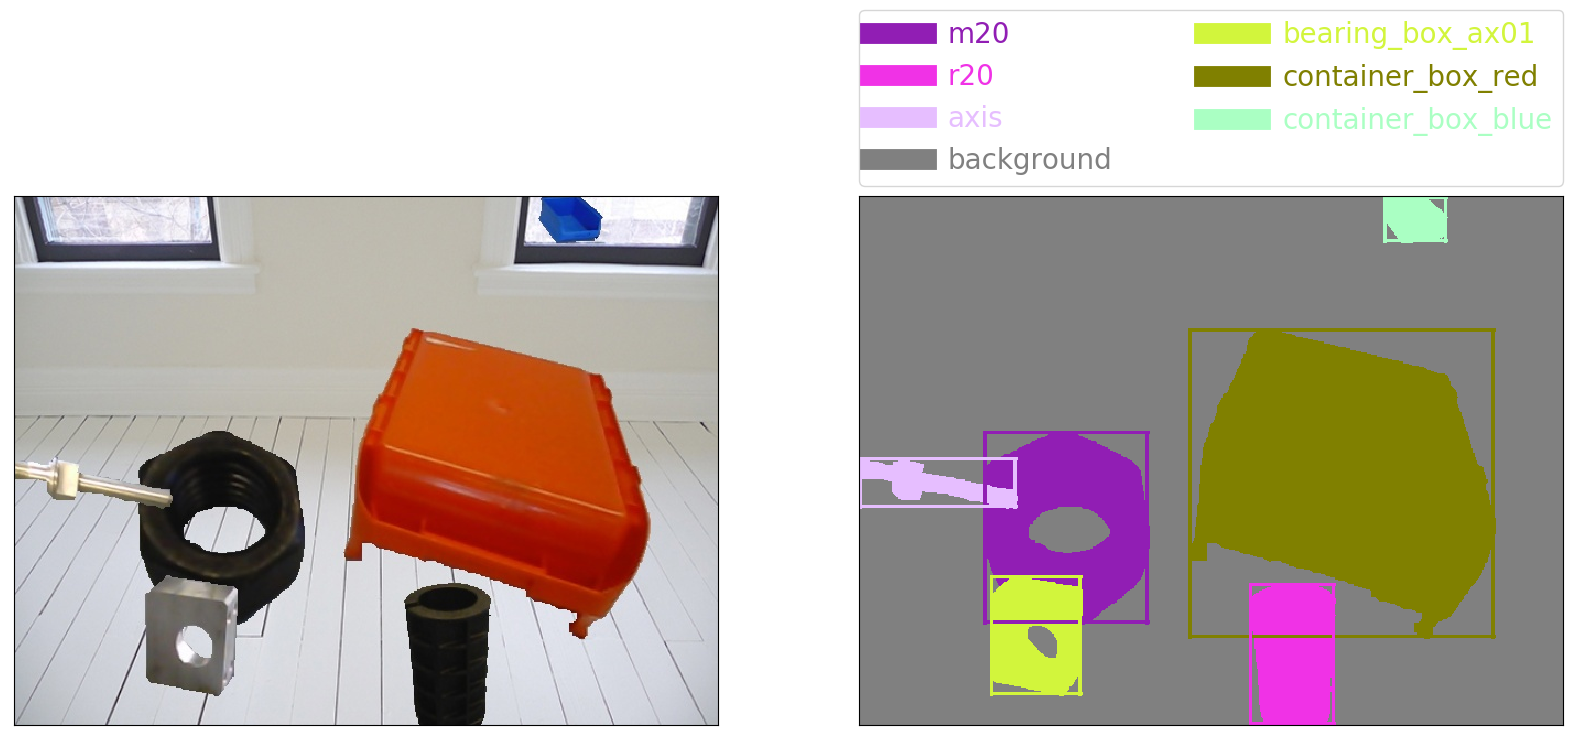
\includegraphics[scale=0.3]{images/sample_white_2}
		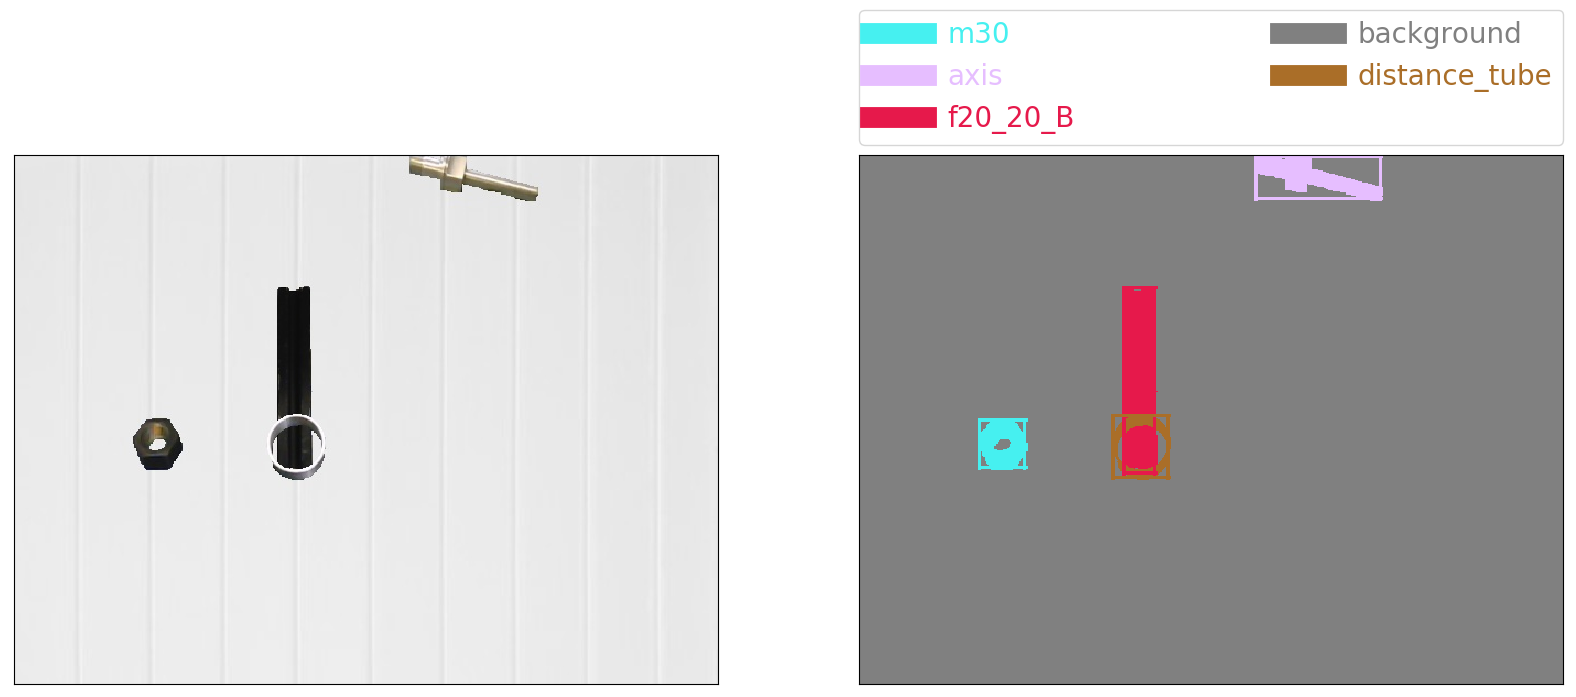
\includegraphics[scale=0.3]{images/sample_white_3}
		\caption{Sample results produced by the artificial image generation algorithm for the "white backgrounds dataset".}
		\label{Fig:samplewhite}
	\end{figure}
	
\section{Data analysis}
\label{section:analysis}
	All the variants of the dataset are analyzed in terms of the pixels occupied by each class in percentage and the number of images in which each class appears.
	
	\subsection{Surface area of the objects}
		
		In order to comprehend the reasons as to why an object constitutes a certain percentage of pixels in a dataset split, the surface area of the objects in the real world could be considered. It is natural to assume that the percentage of pixels occupied by the objects is roughly proportional to the surface area of the object. However, not all objects have a strictly defined geometric shape. For this reason, the closest geometric shape to each object is assumed to calculate the surface area. The table provides details about the assumed geometric shapes and the surface areas for each object.
		
		\begin{table}
			\centering
			\begin{tabular}{|c|c|c|c|c|c|c|c|}
			\hline 
  			\textbf{Object name} & \textbf{Assumed shape} & \textbf{Surface area} \\ 
			\hline
  			 f20\_20\_B & cuboid &  \\ 
			\hline
  			 s40\_40\_G & cuboid &  \\ 
			\hline
  			 f20\_20\_G & cuboid &  \\ 
			\hline
  			 s40\_40\_G & cuboid &  \\ 
			\hline
  			 m20\_100 &  &  \\ 
			\hline
  			 m20 &  &  \\ 
			\hline
  			 m30 &  &  \\ 
			\hline
  			 r20 &  &  \\ 
			\hline
  			 bearing\_box\_ax01 &  &  \\ 
			\hline
  			 bearing &  &  \\ 
			\hline
  			 axis &  &  \\ 
			\hline
  			 distance\_tube &  &  \\ 
			\hline
  			 motor &  &  \\ 
			\hline
  			 container\_box\_blue &  &  \\ 
			\hline
  			 container\_box\_red &  &  \\ 
			\hline
  			 bearing\_box\_ax16 &  &  \\ 
			\hline
  			 em\_01 &  &  \\ 
			\hline
  			 em\_02 &  &  \\ 
			\hline
			\end{tabular}
			\caption{Assumed shape and surface area of objects} 
			\label{Table:surface}
		\end{table}
		
	\subsection{Analysis of "atWork\_full" variant}
		The total pixels occupied by each class in each of the training, validation and test sets is calculated. Next, this count of pixels is converted to percentage with respect to the total number of pixels in the corresponding dataset split. Also, the number of images in which each class of objects appears is counted and called class count. The resulting plots are shown in \ref{Fig:ana_full_b} and \ref{Fig:ana_full}. In \ref{Fig:ana_full_b}, it is evident that compared to the background class, the object classes occupy almost negligible pixel area. This is desired as the background class is present in all images and in most of them, occupies the most pixel area. The larger object classes occupy the most pixel area as can be seen in \ref{Fig:ana_full}. However, in terms of class count all objects are fairly close to each other. A direct reason is infact that larger size occupies more pixel area. Indirectly however, the larger objects are less likely to be rejected by the artificial image generation algorithm after being randomly scaled. This again leads to increased pixel area occupied by the larger objects.
			
			\begin{figure}
			\centering
				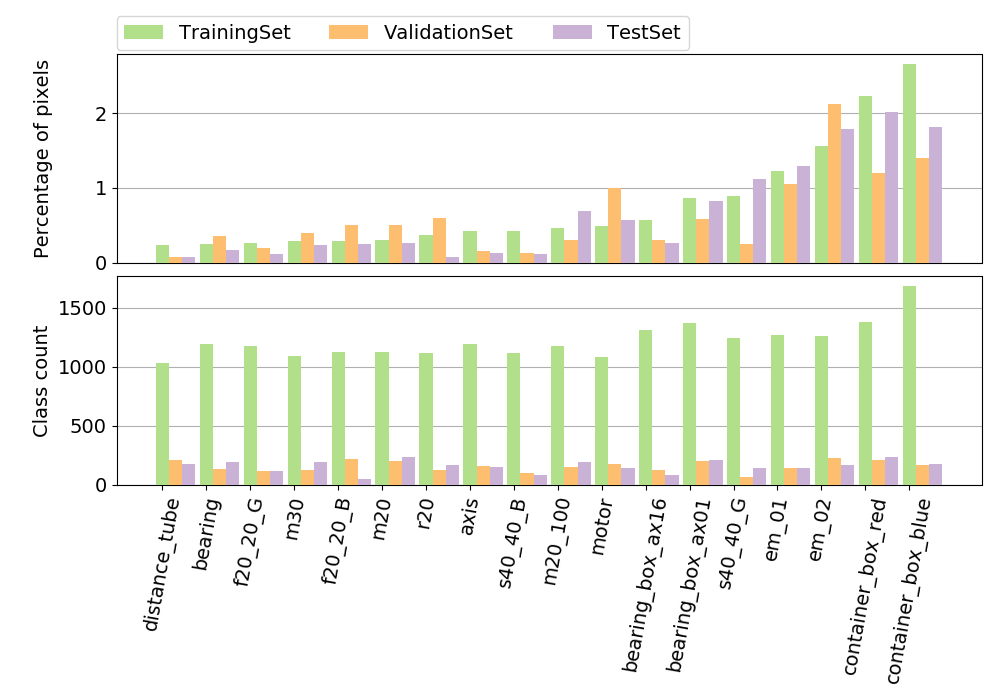
\includegraphics[scale=0.5]{images/full_noB}
				\caption{Percentage of pixels occupied by every class, except the background class, and corresponding class counts in the atWork\_full variant. The larger objects such as "container\_box\_blue" occupy more number of pixels in comparision to smaller objects such as "distance\_tube".}
				\label{Fig:ana_full}
			\end{figure}
		
	\subsection{Analysis of "atWork\_size\_invariant" variant}
		
		\begin{figure}
		\centering
			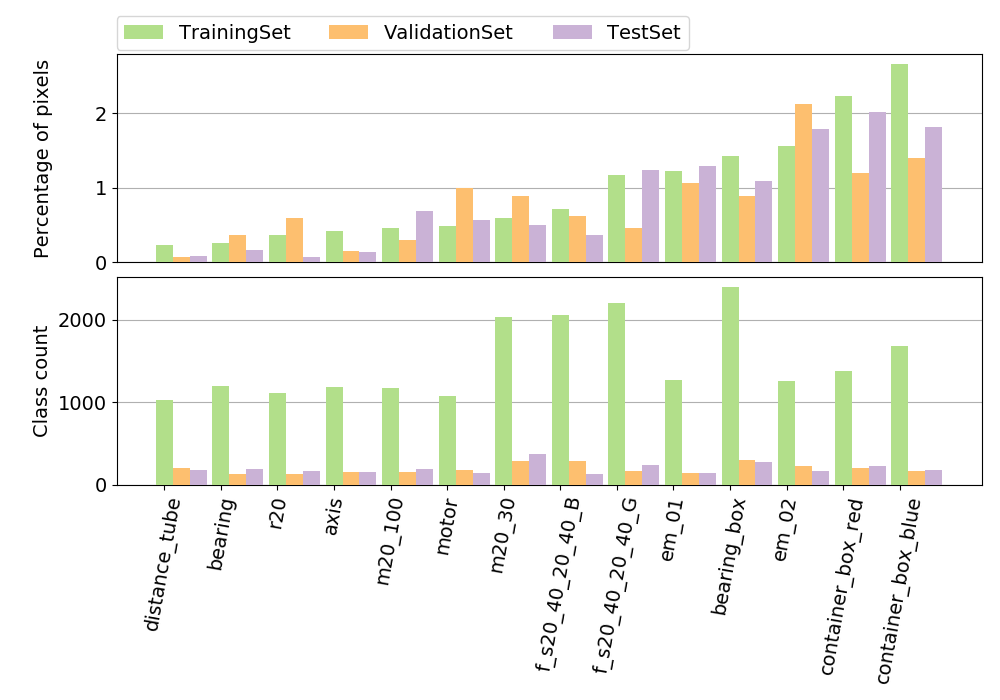
\includegraphics[scale=0.5]{images/size_noB}
			\caption{Percentage of pixels occupied by every class, except the background class, and corresponding class counts in the atWork\_size\_invariant variant.}
			\label{Fig:ana_size}
		\end{figure}
		
	\subsection{Analysis of "atWork\_similar\_shapes" variant}
		
		\begin{figure}
		\centering
			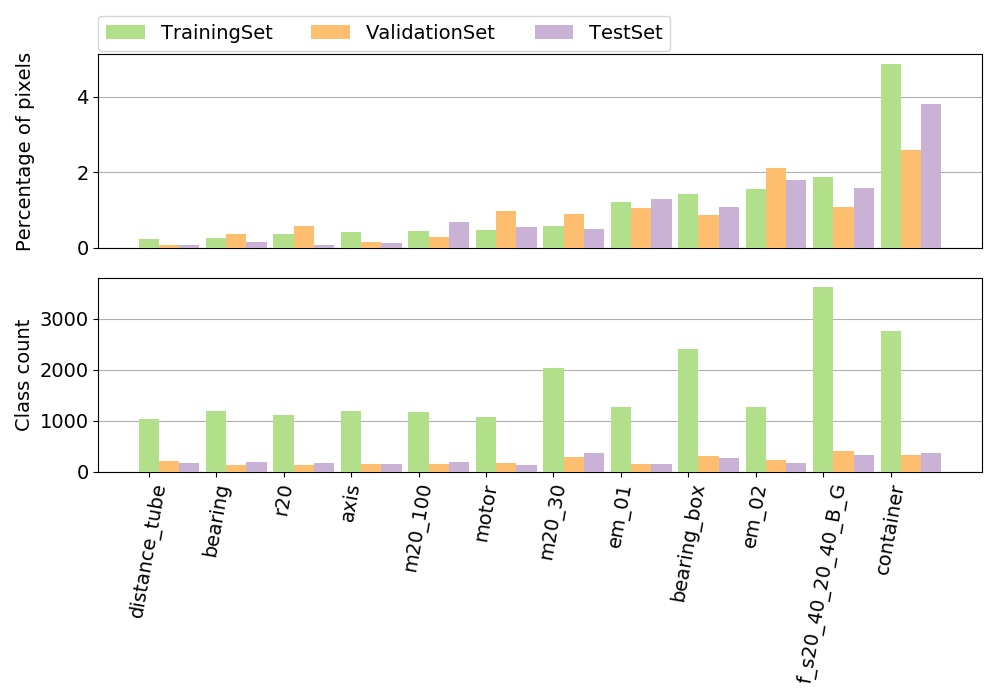
\includegraphics[scale=0.5]{images/shape_noB}
			\caption{Percentage of pixels occupied by every class, except the background class, and corresponding class counts in the atWork\_similar\_shapes variant.}
			\label{Fig:ana_shape}
		\end{figure}
		
	\subsection{Analysis of "atWork\_binary" variant}
	

\newpage
\section{Meta-data of the dataset}

Meta-data of the dataset is provided in Table \ref{Table:meta}. These numbers hold true for all four dataset variants and also for the shades of white dataset. Initially, 30 images were captured for each of the 18 objects leading to a total of 540 images. However, 1 image of "axis" object and 2 images of "s40\_40\_B" were removed as they were blurred.

\begin{table}
	\centering
	\begin{tabular}{|c|c|c|c|c|c|c|c|}
	\hline 
    & Training & Validation & Test \\ 
	\hline 
	Real Images & \makecell{22 per object.\\ Total: 22$\times$18=396} & \makecell{4 per object.\\ Total: 4$\times$18=72} & 				\makecell{"axis"=3; \\"s40\_40\_B"=2; \\All other objects=4\\ Total: (4$\times$18)-3=69} \\ 
	\hline 
	Artificial Images & 7104 & 870 & 870 \\ 
	\hline 
	Total Images & 7500 & 942 & 939 \\ 
	\hline 
	\end{tabular}
	\caption{Meta-data of all 4 variants of the variety of backgrounds and the white backgrounds dataset.} 
	\label{Table:meta}
\end{table}

\section{Possible directions of improvement}

Creating a custom dataset for a desired application is evidently challenging. To overcome the time consuming nature of creating annotations for semantic segmentation, choices such as 1. placing just 1 object per image while taking real images and 2. augmenting the objects on a random selection of diverse backgrounds, were made. This method of augmentation, although inspired by dataset generation method used in \cite{DBLP:journals/corr/abs-1709-00849} and the Synthia dataset \cite{RosCVPR16}, takes a different approach. Unlike \cite{DBLP:journals/corr/abs-1709-00849}, which uses 3D CAD models, this approach does not require any 3D models. Also, this approach does not require a virtual world as used by the Synthia dataset \cite{RosCVPR16}. 
The following list provides possible directions of improvement:
	\begin{itemize}
		\item The ImageLabeler app by default saves the label '.png' file with the name 'Label\_1.png' in a folder called PixelLabelData. A automation script can be written and added to the ImageLabeler to provide options to save the label file in a way the user wants.
		\item Creating a way to replace all unlabeled pixels with the label value of 'background' from within the ImageLabeler would be helpful. For now, this is done by first exporting the label, then loading the label using opencv in python to replace 0 (value of unlabeled pixels) with 19 (value of 'background').
		\item The artificial image generation algorithm is written in python and is independent of the MATLAB ImageLabeler app. This can be improved by including a way to start artificial image generation right from the ImageLabeler.
	\end{itemize}

